\documentclass[12pt,draftclsnofoot,journal,onecolumn]{IEEEtran}
% documentclass[journal, twocolumn]{IEEEtran}
\usepackage{amsfonts}
\usepackage{amsmath,amssymb}
\usepackage{acronym}  % make an acronym
\usepackage{algorithm}
\usepackage{algorithmic}
\usepackage{balance}
\usepackage{bm}
\usepackage{bbm}
\usepackage{booktabs}
\usepackage{color, soul}
\usepackage{cite}
\usepackage{flushend}
\usepackage{graphicx}
\usepackage{indentfirst}
\usepackage{setspace}
\usepackage{tikz}
\usetikzlibrary{arrows}
\usepackage{subfigure}
\usepackage[amsmath,thmmarks]{ntheorem}
\usepackage{theorem}
% Enable Hyper-references.
\usepackage{hyperref}
\hypersetup{hidelinks, 
colorlinks=true,
allcolors=black,
pdfstartview=Fit,
breaklinks=true}

\newtheorem{theorem}{\bf Theorem}
\newtheorem{proposition}{\bf Proposition}
\newtheorem{lemma}{\bf Lemma}
\newtheorem{definition}{Definition}
\newtheorem{remark}{\bf Remark}

\theoremheaderfont{~~~\it}\theorembodyfont{\upshape}%
\theoremstyle{nonumberplain}
\theoremseparator{}
\theoremsymbol{\rule{1ex}{1ex}}
\newtheorem{proof}{Proof:}
\acrodef{SNR}[SNR]{signal-to-noise ratio}
\acrodef{DoF}[DoF]{degree of freedom}
\acrodef{FPGA}[FPGA]{field programmable gate array}
\acrodef{RF}[RF]{radio-frequency}
\acrodef{BS}[BS]{base station}
%\acrodef{RIS}[RIS]{reconfigurable intelligent surface}
%do not use \ac{RIS}
\acrodef{DL}[DL]{downlink}
\acrodef{TA}[TA]{transmit antenna}
\acrodef{RA}[RA]{receive antenna}
\acrodef{LoS}[LoS]{line-of-sight}
\acrodef{RC}[RC]{receiver combining}
\acrodef{AWGN}[AWGN]{additive white Gaussian noise}
\acrodef{DFT}[DFT]{discrete Fourier transform}
\acrodef{IRF}[IRF]{interference random field}
\acrodef{MISO}[MISO]{multiple-input single-output}
\acrodef{CSI}[CSI]{channel state information}
\acrodef{CRLB}[CRLB]{Cramer-Rao lower bound}
\acrodef{UPA}[UPA]{uniform planar array}

\def \H {^H}
\def \opt {^{\text{opt}}}
\def \v {\bm v}
\def \w {\bm w}
\def \g {\bm g}
\def \f {\bm f}
\def \T {\bm \Theta}
\def \t {\bm \theta}
\def \x {\bm \xi}
\def \Pmax {P_{\text{max}}}
\def \ml {multi-layer }
\def \tb {transmit beamformer }
\def \sl {single-layer }
\def \diag {\text{diag}}
\def \opt {^{\text{opt}}}
\def \exp {\text{exp}}
\def \arg {\text{arg}}
\def \CN {\mathcal{CN}}
\def \VM {\mathcal{VM}}
\def \re {\text{Re}}
\def \nc {\mathcal{NC}}
\def \ch {\textcolor{red}{(cite here) }}

\newcommand{\RNum}[1]{\uppercase\expandafter{\romannumeral #1\relax}}
\renewcommand{\algorithmicrequire}{\textbf{Input:}}   %Use Input in the format of Algorithm
\renewcommand{\algorithmicensure}{\textbf{Output:}}  %UseOutput in the format of Algorithm
\newcommand{\myincludegraphics}[2][width=12cm]{\includegraphics[#1]{#2}}
% 12cm for onecolumn,

\ifCLASSINFOpdf
\else
\fi
\hyphenation{op-tical net-works semi-conduc-tor}
\begin{document}
\title{Sensing RIS: Enabling Dimension-Independent CSI Acquisition for Beamforming}
\author{{Jieao~Zhu, Kunzan~Liu, Zhongzhichao~Wan, Linglong~Dai, {\textit{Fellow, IEEE}, \\and H.~Vincent~Poor, {\textit{Life Fellow, IEEE}}}
\vspace*{-3em}}
\thanks{J. Zhu, K. Liu, Z. Wan, and L. Dai are with the Beijing National Research Center for Information Science and Technology (BNRist) as well as the Department of Electronic Engineering, Tsinghua University, Beijing 100084, China (e-mails: \{zja21, lkz18, wzzc20\}@mails.tsinghua.edu.cn, daill@tsinghua.edu.cn).

H. V. Poor is with the Department of Electrical and Computer Engineering, Princeton University, USA (e-mail: poor@princeton.edu).

This work was supported in part by the National Key Research and Development Program of China (Grant No.2020YFB1807201), in part by the National Natural Science Foundation of China (Grant No. 62031019), and in part by the European Commission through the H2020-MSCA-ITN META WIRELESS Research Project (Grant No. 956256).}
}

\maketitle

\begin{abstract}
Reconfigurable intelligent surface (RIS) has been envisioned as a revolutionary paradigm for future wireless communications.
However, the RIS's disability of processing signals and the increased channel dimension have brought new challenges to RIS-assisted system, which greatly increases the pilot overhead required for channel estimation.
To tackle this problem, several prior contributions that enhance the hardware architecture of RIS or develop algorithms to exploit the channels' mathematical properties have been made, where the required pilot overhead is reduced to be proportional to the number of RIS elements.
In this paper, we propose a dimension-independent channel state information (CSI) acquisition approach, that the required pilot overhead is independent of the number of RIS elements.
Specifically, in contrast to traditional signal transmission method, where signals from the base station (BS) and the users are transmitted in different time slots, we propose a novel method that signals are transmitted from the BS and the user simultaneously during CSI acquisition.
Under this method, we reveal the phenomenon that an electromagnetic interference random field (IRF) will occur on RIS, and we employ sensing RIS to capture its feature.
Moreover, we develop three algorithms for parameter estimation in this system, and also derive the Cramer-Rao lower bound (CRLB) and its asymptotic expression.
Simulation results verify that our proposed signal transmission method and the corresponding algorithms can achieve dimension-independent CSI acquisition for beamforming.
\end{abstract}

\begin{IEEEkeywords}
Reconfigurable intelligent surface (RIS), channel estimation, interference random field (IRF), dimension-independent CSI acquisition. 
\end{IEEEkeywords}

\section{Introduction}
Reconfigurable intelligent surface (RIS) has been envisioned as a revolutionary paradigm for future wireless communications.
The characteristics of low cost and power consumption provide RIS with promising applications in overcoming blockages, improving capacity, and reducing transmit power \cite{basar2019wireless,liu2021compact,wu2019intelligent}.
Specifically, RIS is a large-scale array composed of passive elements, which can achieve significant beamforming gain by appropriately imposing the phase shifts on the incident electromagnetic waves \cite{di2020smart}.
To achieve this beamforming gain, accurate \ac{CSI} should be acquired beforehand, which makes channel estimation an essential problem for RIS-assisted communications \cite{wei2021channel}.

Although channel estimation has been well investigated in conventional communication systems, the additional employment of RIS brings about two challenges \cite{weili2021channel}.
Firstly, in contrast to the traditional antenna array capable of transmitting, receiving, and processing the signals, RIS can only passively reflect the incident signals.
Secondly, since the number of RIS elements is usually large, the dimensions of the channels increase sharply compared with conventional communication systems, which results in unacceptably high pilot overhead for channel estimation.
These two main challenges result in the urgent need for new channel estimation techniques for beamforming in RIS-assisted communications.

\subsection{Prior Works}
\label{Prior Works}
% Add here
Generally, for RIS-assisted systems, channel estimation and beamforming are two separate procedures.
Channel estimation is performed first, and then the obtained \ac{CSI} is utilized for beamforming.
The beamforming gain highly relies on the channel estimation accuracy.

To tackle the challenges mentioned above in channel estimation for RIS-assisted communications, some solutions have been recently proposed, which can be generally divided into two categories.
The first category modifies the hardware architecture of RIS, which enables a little bit of signal processing capability.
For example, by sparsely replacing some of the RIS elements with active sensors capable of baseband processing, the authors of \cite{taha2021enabling} proposed a compressive sensing and deep learning-based channel estimation scheme with negligible pilot overhead. 
To further reduce the number of active sensors, in \cite{alexandropoulos2020hardware} the authors proposed an alternating direction method-based channel estimation procedure with a single \ac{RF} chain, with the help of an extended analog combiner \cite{vlachos2019wideband}. Since RF chains have been attached to RIS for channel sensing in these works, they can also be modified to perform signal relay. In \cite{nguyen2021hybrid}, a hybrid relay-reflecting architecture is considered, where a few passive RIS elements are replaced by the active amplify-and-forward relay modules. These active modules are then capable of channel estimation. 

The second category preserves the original hardware architecture of RIS, while conceiving new algorithms to exploit the specific features that RIS brings about.
Exploiting the two-timescale channel property in the RIS-assisted system, the authors of \cite{Huchen} proposed a two-timescale channel estimation algorithm that reduces the pilot overhead in the time-averaged sense.
In other works \cite{wang2020compressed,wei2021channel}, by exploiting the sparsity of channels in the angular domain, compressive sensing-based algorithms are developed with reduced pilot overhead.
In \cite{wang2020channel}, based on the shared reflected channels among multi-users, the authors proposed a three-phase channel estimation framework to further reduce the pilot overhead. 
% In \cite{kundu2021channel}, deep learning approaches are considered to improve the performance of estimation.
% Multi-user relevance, two-timescale channel property & channel sparsity. 

%% Re-interpret. All the above methods require channel matrix first. The channel matrix is at least of size O(N). Usually...
Note that, in order to achieve high beamforming gain, all the above classical channel estimation methods are designed to estimate the full channel matrix as accurately as possible. However, since the channel matrix is at least of size $\mathcal{O}(N)$, where $N$ denotes the number of RIS elements, the required pilot overhead for channel estimation is usually proportional to the number of RIS elements \cite{taha2021enabling,alexandropoulos2020hardware,nguyen2021hybrid,Huchen,wang2020compressed,kundu2021channel} in practical systems, which makes most of the existing channel estimation schemes dimension-dependent. This is unacceptable especially when the RIS is fabricated with larger number of elements (e.g. 1100 elements in \cite{pei2021ris}, 2304 elements in \cite{yangfan2020coding}, and 10240 elements in \cite{yang2018reconfigurable}).   % larger RIS! fabricated (how many elements?)
Therefore, the question naturally arises as: {\it Does there exist a dimension-independent approach where the required pilot overhead is independent of the number of RIS elements?}

% In a nutshell, both the above two categories have two limitations:
% \begin{enumerate}
% \item[1)]  Channel estimation only extracts the mathematical features of channels, while neglects their electromagnetic nature.
% \item[2)] The procedure of channel estimation and beamforming are separated, where redundant information is needlessly estimated.
% \end{enumerate}

\subsection{Our Contributions}
\label{Our Contributions}

We point out that the main drawback of conventional channel estimation methods is that they only extract the mathematical features of channels, while neglect their electromagnetic nature. This limitation has caused the problem of high pilot overhead required for channel estimation in RIS-assisted systems. Thus, we propose an \ac{IRF}-based approach, where the \ac{IRF} on RIS is utilized for channel estimation\footnote{Simulation codes will be provided to reproduce the results in this paper: \url{http://oa.ee.tsinghua.edu.cn/dailinglong/publications/publications.html}.}.
Specifically, the contributions of this paper can be summarized as follows.
    \begin{itemize}
        \item %We propose a novel signal transmission framework in RIS-assisted system, and reveal the corresponding phenomenon of electromagnetic interference.
        % up-link channel estimation / down-link channel estimation
        Inspired by optical interference where phase information can be obtained from the interference fringes, we reveal that phase information about the channel can also be gathered from the phenomenon of electromagnetic interference that occurs on RIS, which we name as the \ac{IRF}. %Fortunately, phase information is enough for RIS beamforming that serves a single-antenna user. 
        To create the \ac{IRF} on RIS, we propose a novel pilot transmission method called simultaneous rotational signaling, where signals are transmitted from the \ac{BS} and the user to RIS simultaneously, and the two signals bear a slight frequency difference during CSI acquisition. 
        \item
        To exploit this \ac{IRF} for CSI acquisition, we employ sensing RIS which integrates power detectors into the RIS elements to capture the features of the \ac{IRF}. Each of the power detectors can acquire its phase information independently from the \ac{IRF}, so that the required pilot overhead is independent of the number of RIS elements. 
        We then develop DFT, ML, and VM-EM phase estimation algorithms to extract the phase information from the power detector signals in order to perform beamforming. 
        \item
        We derive the \ac{CRLB} of the phase estimation problem based on the \ac{IRF}, and its approximated asymptotic expression for channel estimation in the sensing RIS-assisted system.
        Our numerical results verify that this approximated \ac{CRLB} is asymptotically precise, and that our developed algorithms are close to \ac{CRLB}. 
        Our simulation results further demonstrate that our proposed signal transmission method and the corresponding algorithms can realize dimension-independent CSI acquisition for beamforming, and then achieve the near-optimal spectral efficiency. 
        
%        The \ac{IRF} generated by the BS and UE makes it possible to obtain CSI with only one pilot symbol. Thus, the pilot overhead is reduced to $\mathcal{O}(1)$, independent of the number of RIS elements $N$. 
%        \item After measuring the \ac{IRF} by the integrated power sensors, it is possible to directly calculate the optimal phase for each RIS element within $\mathcal{O}(1)$ time. However, traditional channel estimation schemes require at least $\mathcal{O}(N)$ time, since the scale of the estimation problem is at least $\mathcal{O}(N)$.
%        \item Both the CSI acquisition and beamforming can be done immediately at the RIS, thus making channel feedback and BS signal processing unnecessary.
%        \item Compared to attaching RF chains to the RIS elements\cite{zhang2021channel}, power sensors are much more cost-efficient and energy-efficient, since power sensors do not include LNAs, mixers and complicated baseband signal processors which turn out to be  essential for RF chains.
%        \item The \ac{IRF} channel estimation and beamforming method is not affected by near-field effect, since this method does not rely on the prior knowledge of how the BS-RIS and RIS-user channels are structured. 
    \end{itemize}

\subsection{Organization and notation}

\textit{Organization:}
The rest of the paper is organized as follows.
In Section~\ref{System Model}, we introduce the system model of RIS-aided communications, and review the traditional separate procedures of beamforming and channel estimation.
In Section~\ref{Interference Random Field}, we propose a novel signal transmission method for CSI acquisition in RIS-aided system, and reveal the \ac{IRF} phenomenon under this method.
In Section~\ref{Sensing RIS-Based Channel Estimation}, we introduce the hardware architecture of sensing RIS to exploit the \ac{IRF}.
Based on sensing RIS, we propose three algorithms to realize channel estimation.
In Section~\ref{Performance Analysis}, we derive the \ac{CRLB} and its asymptotic expression for channel estimation in the sensing RIS-assisted system.
In Section~\ref{Simulation Results}, simulation results are provided for quantifying the performance of our proposed sensing RIS-based channel estimation as a dimension-independent approach.
Finally, in Section~\ref{Conclusion}, we provide our conclusions followed by promising future research ideas.

\textit{Notation:} $\mathbb C$ and $\mathbb R$ denote the set of complex and real numbers, respectively;
$\{L\}$ represents the set of integers $\{0,1,\cdots,L-1\}$;
$\bm A^{-1}, \bm A^*,\bm A^T,$ and $\bm A^H$ denote the inverse, conjugate, transpose, and conjugate transpose of matrix $\bm A$, respectively; 
$\Vert \cdot\Vert_{2}$ is the $\mathcal{L}_{2}$-norm of its argument function;
$\Vert \cdot \Vert_{F}$ denotes the Frobenius norm of its argument matrix;  
%$\left\langle\bm x\right\rangle$ is the normalized vector of $\bm x$, i.e., $\left\langle\bm x\right\rangle=\bm x/\Vert\bm x\Vert_{2}$;
$\text{arg}(x)$ and $\text{exp}(x)$ denote the phase angle and exponential representation of the complex scalar $x$, respectively;
$\vert x\vert$ denotes the amplitude
of a complex scalar $x$; 
$\text{diag}(\cdot )$ is the diagonal operation;
$\mathcal{CN}\left(\mu, \sigma^2 \right)$ represents the complex univariate Gaussian distribution with the mean $\mu$ and the variance $\sigma^2$;
$\VM(\mu, \kappa)$ denotes the von Mises distribution with circular mean $\mu\in [0,2\pi]$ and centrality $\kappa$;
$\nc_{\chi_k^2}(\lambda, \sigma^2)$ and $\nc_{\chi_k}(\lambda)$ are the degree-$k$ non-central chi-squared distribution with  non-centrality parameter $\lambda$ and variance parameter $\sigma^2$, and the non-central chi distribution with non-centrality parameter $\lambda$, respectively; 
%$\bm 0_{L}$ denotes the $L\times 1$ zero vector;
$\bm I_{L}$ denotes the $L\times L$ identity matrix;
% $\bm \psi_{\text{max}}(\bm A)$ is the eigenvector of matrix
% $\bm A$ corresponding to its largest eigenvalue.
%$\wedge$ and $\vee$ denote logical conjunction and logical
%disjunction, respectively.
$x_{\rm BB}(t)$ denotes the baseband representation of a passband signal $x(t)$;
$I_\nu(z)$ is the $\nu$-th order modified Bessel function of the first kind. 


\section{System Model}  \label{System Model}
    In this section, we will first specify the system model of the RIS-assisted \ac{MISO} system.
    Then, we will introduce traditional approaches for the corresponding beamforming design and channel estimation in Subsection~\ref{Beamforming design} and \ref{Channel Estimation}, respectively.

   % \subsection{RIS-Aided MISO System}  \label{MISO case}
        Let us consider a RIS-aided MISO system, where an $N$-element RIS is employed for enhancing the transmission from an $M$-antenna \ac{BS} to a single-antenna user. Assume furthermore that the phase-shift of RIS's each element can be continuously and independently controlled \cite{wu2019intelligent}. Then, the RIS precoding matrix can be represented by $\bm \Theta = \diag \left(\bm \theta\right )=\diag \left(\left[\theta_{1},\cdots ,\theta_{N}\right]^{T}\right)$,
        where $\theta_n (n\in[N])$ denotes the phase-shift of the $n$-th RIS element, satisfying $\lvert \theta_n\rvert=1$. Therefore, the signal received by the user can be written as 
        \begin{equation}
            \label{Signal model}
            y=\bm f^{H} \bm\Theta \bm G \bm w s+z,
        \end{equation}
        where $\bm f\in \mathbb C ^{N\times 1}$ and $\bm G \in \mathbb C^{N\times M}$ denote the channel spanning from the RIS to the user and the channel spanning from the BS to the RIS, respectively; $\bm w\in \mathbb C^{M\times 1}$ denotes the beamforming vector at the transmitter BS, with power constraint $\left\Vert \bm w\right \Vert_{2}^{2}\leq P_{\text{max}}$; $s$ denotes the normalized BS transmitted symbol; $z\sim \mathcal{CN}\left(0,\sigma_{z}^{2}\right)$ denotes the \ac{AWGN} introduced at the receiver user. To focus on RIS beamforming, other possible links are neglected in this paper\footnote{In fact, our proposed CSI acquisition procedure automatically works when there exists extra links, which will be explained later in this paper.}.
        % TODO: Explain it. 
        
        \subsection{Beamforming Design}
        \label{Beamforming design}
        Based on the received signal \eqref{Signal model}, we can formulate the \ac{SNR} maximization problem for designing the beamforming vector $\bm w$ and precoding matrix $\bm \Theta$, i.e.,
        \begin{subequations}
\label{optimization}
\begin{align}
\label{objective}
\max_{\bm \Theta}~~&\text{SNR}=\frac{1}{\sigma_{z}^{2}}
\left\vert
\bm f^{H}\bm \Theta\bm G\bm w \right\vert^{2},\\
\label{constraint}
~~~~~\text{s.t.~~~}&\text{C}_{1}: \left\Vert \bm w\right \Vert_{2}^{2}\leq P_{\text{max}},\\
&\text{C}_{2}: \left\vert\theta_{n}\right\vert=1,~\forall n.
\end{align}
\end{subequations}
        
        
        In this paper, we assume that the locations of the \ac{BS} and the RIS are unchanged, which can provide us a beamforming approach expressed as
                \begin{equation}
\label{traditional beamforming}
\bm w=\sqrt{P_{\rm max}}\bm a\left(\alpha\right),\quad \theta_{n} = \exp\left(-{\rm j} \arg\left(f_{n}^{*}\bm g_{n}^{T}\bm w\right)\right),~\forall n\in \{N\},
\end{equation}
where $\bm a(\alpha)$ denotes the array steering vector with respect to the wave departure angle $\alpha$ of the BS antenna array, and $\bm G = \left[\bm g_{1}, \cdots, \bm g_{N}\right]^{T}$.

\subsection{Channel Estimation}
\label{Channel Estimation}
    Observe from \eqref{traditional beamforming} that, the estimation for the cascade channel ${\bm H} = {\rm diag}({\bm f}^{*})\bm G$ is enough for beamforming design.
    To accurately acquire this cascade channel, the user generally sends pilot signal $x$ to the BS under $P$ different RIS configurations which are the first $P$ columns of the DFT matrix $\bm F_N$, denoted as $\bm F_{N,P}$. 
    Due to the channel reciprocity, the received signal at the BS with the $p$-th RIS configuration $\bm \Theta_{p}=\diag({\bm \theta}_p)$ can be written as \cite{atapattu2020reconfigurable}
    \begin{equation}
    \label{CE received signal}
        {\bm y}_{{\rm BS}, p} =\bm H^{T} {\bm \theta}_p w' s'+\bm n,
    \end{equation}
    where $w'$ is the precoding scalar of the user satisfying $|w'|^2 \leq P_{\rm max}'$, $s'$ is the normalized user transmitted symbol, and $\bm n\sim \mathcal{CN}\left( \bm 0_{M}, \sigma_{n}^{2}\bm I_{M}\right)$ is the \ac{AWGN} at the receiver BS.
    Equivalently, \eqref{CE received signal} can be expressed in the matrix form
    \begin{equation}
    \label{eqn:LS_CE model}
        {\bm Y}_{\rm BS}=\bm H^{T} \bm F_{N,P}w' s' + {\bm N},
    \end{equation}
    where ${\bm Y}_{\rm BS}=\left[\bm y_{{\rm BS}, 1},\cdots,\bm y_{{\rm BS}, P}\right]$ and $\bm N = \left[ \bm n_{1},\cdots,\bm n_{P}\right]$.
    Given the received signal $\bm Y_{\rm BS}$ and, without loss of generality, assuming $w's'=1$, the channel estimation problem in RIS-assisted system can be formulated as 
    \begin{equation}
        \hat{\bm H} = \arg\min_{\bm H} \lVert {\bm Y}_{\rm BS} - {\bm H^{T}} {\bm F}_{N,P}\rVert_{F}^2.
    \end{equation}
    With the least-square (LS) criterion \cite{kundu2021channel}, we obtain
    \begin{equation}
        \hat{\bm H}_{\rm LS} = \frac{1}{P}{\bm F}_{N,P}^{*}{\bm Y}_{\rm BS}^{T},
        \label{eqn:LS-CE}
    \end{equation}
    which provides a feasible solution to channel estimation in this RIS-assisted MISO system. In this paper, we name it the least-square channel estimation (LS-CE) method. 

\section{Interference Random Field}
\label{Interference Random Field}
    In this section, the signal model for \ac{IRF} will be first introduced in Subsection~\ref{Models for IRFs}. Then, in order to acquire the CSI, the simultaneous rotational signaling method will be proposed in Subsection~\ref{Simultaneous Rotational Signaling and Interference Detection}. 

\subsection{Signal Model for IRF}
\label{Models for IRFs}

    Physical intuition is vital in designing RIS-aided systems \cite{najafi2020physics}, and interference is a fundamental physical phenomenon in all kinds of waves. The most well-known example is the double-slit optical interference \cite{louradour1993interference}, as is shown in Fig.~\ref{fig:scheme}~(a), where the interference fringes created during the wave superposition reveal the phase difference of the two optical paths. Similarly, the same interference phenomenon occurs when two RF electromagnetic waves meet together on the RIS, as is shown in Fig.~\ref{fig:scheme}~(b), and the \ac{IRF} created by this interference unveils the \ac{CSI}. 
    \begin{figure}[t]
        \centering
        \subfigure[Optical interference.]
        {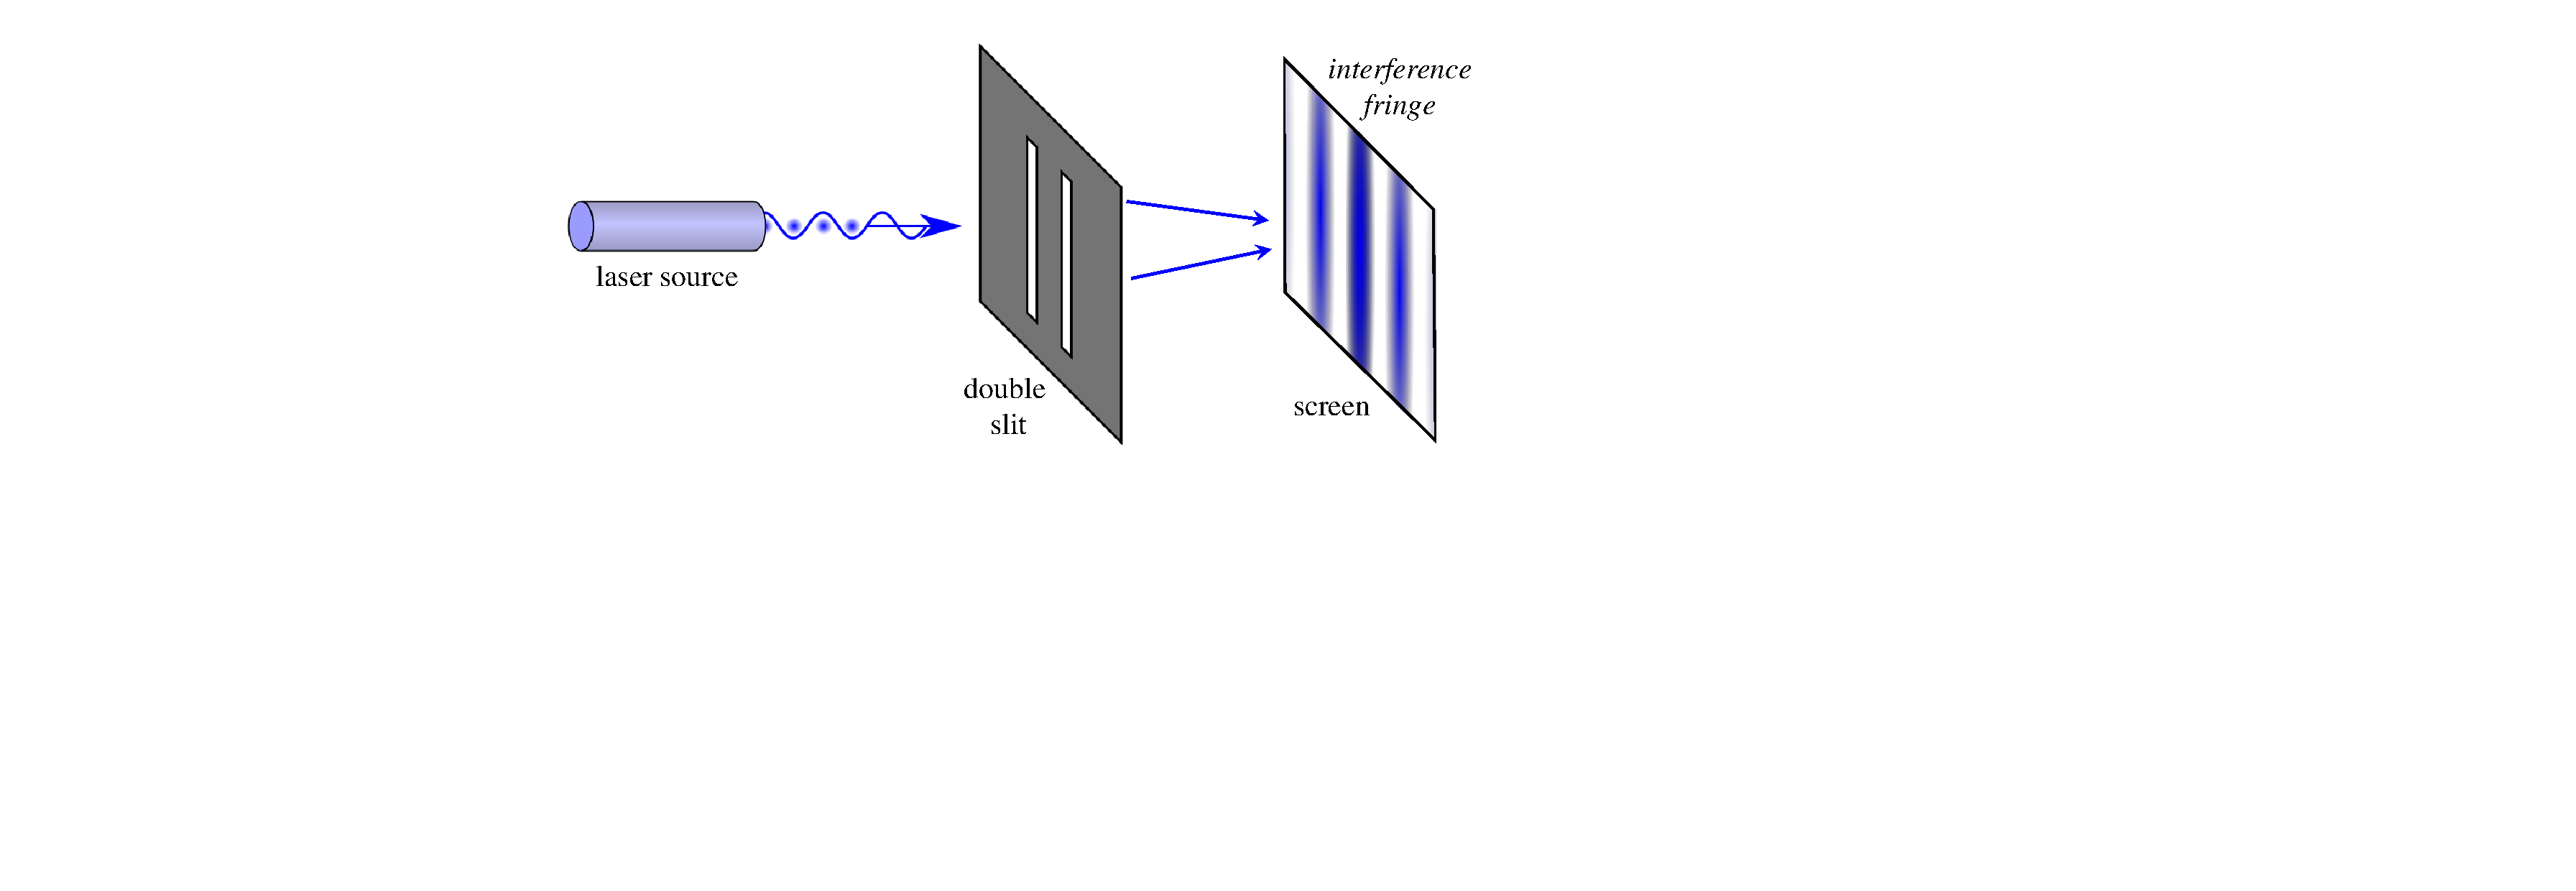
\includegraphics[width=.6\textwidth]{figures/scheme1.pdf}}
        %\vspace{0.2mm}
        \subfigure[Electromagnetic interference.]
        {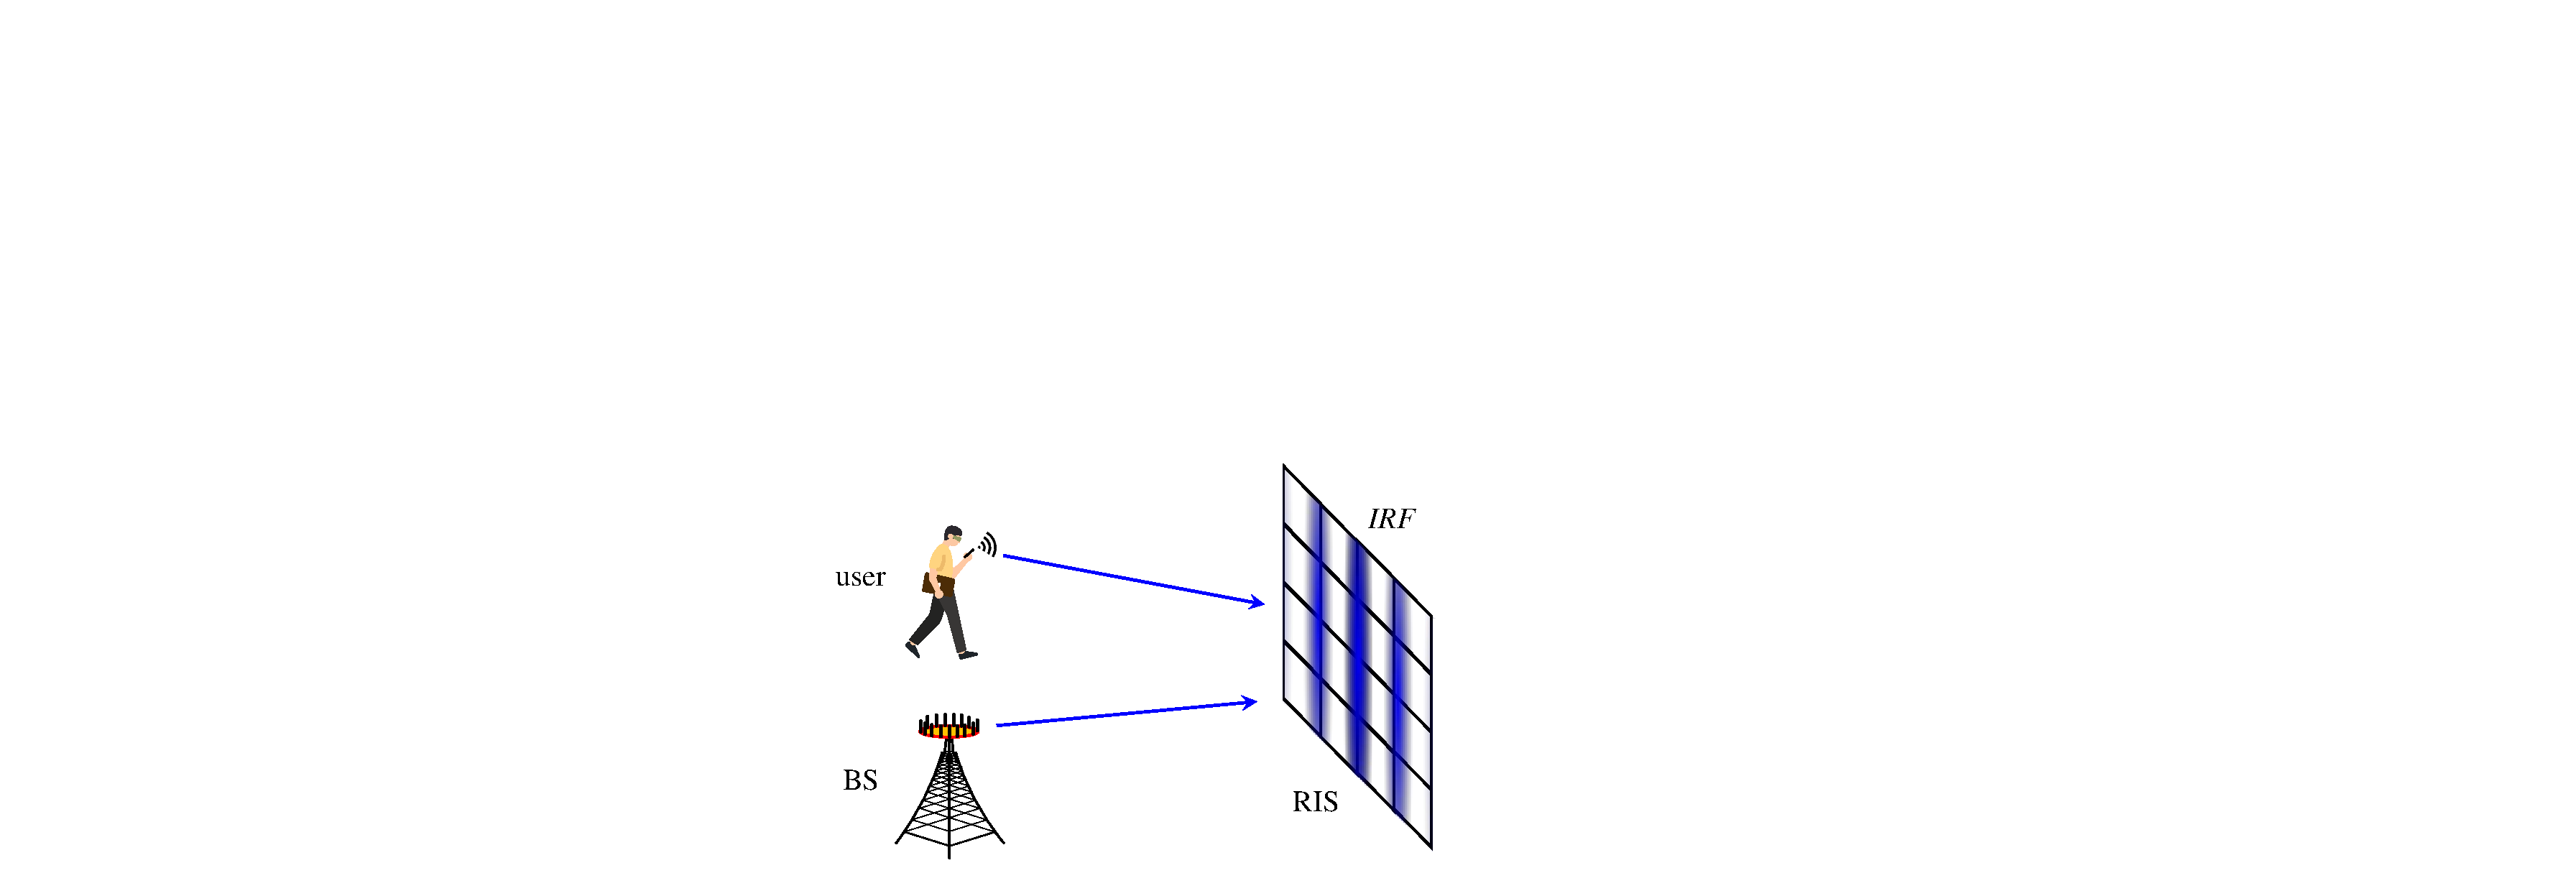
\includegraphics[width=.6\textwidth]{figures/scheme2.pdf}}
        \caption{Analogy between the optical interference and the \ac{IRF} phenomenon occurred on RIS.}
        \label{fig:scheme}
        %\vspace{-0.5em}
    \end{figure}

    Suppose two signals imping the RIS simultaneously, creating an interference field at the $n$-th RIS element. Denote the symbol transmitted from \ac{BS} by $s$, and the symbol transmitted from the user by $s'$. In order to perform channel estimation by exploiting the \ac{IRF}, we need to probe the interference fringes, i.e., the power of the \ac{IRF}. To clarify the power problem associated with an electromagnetic signal, the relationship between physical signal power and baseband equivalent signal power is stressed in the following formulas. 
    If we represent both of the BS-RIS and user-RIS signals that appear on each RIS element by their baseband equivalent signals $E_{{\rm BB}}(t)$, 
    then the corresponding physical passband electric field induced on each RIS element is characterized by 
    \begin{equation}
        E_(t) = \sqrt{2} {\rm Re}\left( E_{{\rm BB}}(t)e^{{\rm j}\omega_c t} \right),
        \label{baseband-passband relationship}
    \end{equation}
    where $\omega_c = 2\pi f_c$ denotes the carrier frequency, and the coefficient $\sqrt{2}$ ensures that the passband signal energy (power) is equal to the baseband signal energy (power), i.e., 
    $\lVert E_{{\rm BB}}\rVert_2^2 = \lVert E\rVert_2^2$. 
    Thus, taking the square of the baseband signal is equivalent to calculating the power of the physical electromagnetic signal. 
    Now we consider the IRF case, where a superposition of the BS-RIS signal and the user-RIS signal is considered. 
    Following the notations in Section~\ref{System Model} and due to the linearity of \eqref{baseband-passband relationship}, we obtain the noisy IRF signal by adding up the two impinging baseband signals
    \begin{equation}
        \begin{aligned}
            E_{{\rm BB, IRF}}(t) &= E_{{\rm BB, BS}}(t)+E_{{\rm BB,user}}(t)+v(t)\\
            &=\bm g_{n}^{T}\bm w s+f_{n}^{*} w' s' +v(t),
        \end{aligned}
    \end{equation}
    where $v(t)\sim \mathcal{CN}(0,\sigma_{v}^{2})$ is the electromagnetic noise signal in its baseband representation, $\bm w$ and $w'$ are the beamforming vector at the BS side and the user side, respectively, which satisfies
    \begin{equation}
    \label{power constraint}
    \Vert \bm w \Vert_{2}^{2}\leq P_{\text{max}}, \quad |w'|^{2}\leq P'_{\text{max}}.
    \end{equation}
    $s$ is the symbol transmitted from the BS to RIS, and $s'=e^{{\rm j} \psi(t)}$ is the time-varying transmitted symbol from the user to RIS.  
    Since the interference fringes are not sensitive to a global phase change, we can safely assume that $s=1$, and then the relative phase between the user and BS can be fully characterized by a time-varying phase function $\psi(t)$.  

    Furthermore, by defining $\alpha = \left\vert\bm g_{n}^{T}\bm w\right\vert$, $\beta = \left\vert f_{n}^{*} w' \right\vert$, and the phase difference between the \ac{BS}-RIS link\footnote{Since it is usually difficult to obtain the optimal BS beamforming vector $\bm w$, during the CSI acquisition procedure, we fix $\bm w$ to a steering vector that guides most of the signal energy to the RIS aperture. As a result, $\bm g_n^T \bm w$ can be treated as the equivalent link seen by the symbol $s$.} and the RIS-user channel as $\varphi = \arg\left(f_{n}^{*}w'\right)-\arg\left(\bm g_{n}^{T}\bm w\right)$, then the power of the \ac{IRF} can be written as
    \begin{equation}
        \label{eqn:power of interference}
        \begin{aligned}
            P(t)&=A \left| E_{{\rm BB, IRF}} (t)\right |^{2}+\zeta\\
            &=\underbrace{A\left[\alpha^{2}+\beta^{2}+2\alpha\beta\cos\left(\psi(t)+\varphi\right)\right]}_{\text{IRF power signal}}\\
            &~~~+\underbrace{2A\text{Re}\left\{\left(\alpha+\beta e^{{\rm j}\left(\psi(t)+\varphi\right)}\right)v'^{*}(t)\right\}+A\left|v'(t)\right|^{2}+\zeta}_{\text{Noise}},\\
        \end{aligned}
    \end{equation}
    where $\zeta$ is the noise introduced by digital signal processing after measuring the IRF power, $A$ is the amplification factor of the power sensor, and the equivalent electromagnetic noise $v'(t) = e^{{\rm j}{\rm arg}({\bm g}_n^T \bm w)}v^*(t)$ follows the same distribution as $v(t)$ for any time $t$.
    The name IRF comes from the randomness of the unknown $\varphi$, the unknown noise realization, and the interferential nature of the field.

    The phase difference $\varphi$ defined here will play an important role in our following channel estimation, since it carries enough CSI for beamforming, which will be justified in the next section. To estimate the phase difference $\varphi$, we need enough observations from the sensor-detected power signal $P(t)$. For simplicity and without loss of generality, we can assume $\psi(t)=\omega t$ and $\omega=\frac{2\pi}{T_{s}}$, where $T_s$ is the symbol period. Furthermore, assume that $L$ observations $P[l]=P(t_{l})$ located at equally-spaced instants 
    \begin{equation}
        \label{observation time}
        t_{l}=\frac{l}{L}T_{s},~\forall l\in \{L\}
    \end{equation}
    are used for phase estimation $\varphi$.

\subsection{Simultaneous Rotational Signaling and Interference Detection} \label{Simultaneous Rotational Signaling and Interference Detection}
    However, at first glance it seems impractical to use only power signals to obtain enough information for RIS beamforming, in the absence of phase information. 
    Generally, signal processing with only amplitude signals are called {\it noncoherent} detection. The target of RIS beamforming is to strengthen the signal at the user, hence it requires {\it coherent} signal combining at the user antenna.  
    As a result, for {\it noncoherent} detection, it seems that the lack of phase information makes beamforming impossible. 
    Fortunately, the physical phenomenon {\it interference} makes it possible to convert phase difference into intensity difference, allowing {\it noncoherent} devices to perform {\it coherent} detection. 
         
    \begin{figure}[!t]
        \centering
        \includegraphics[width=.9\textwidth]{data/protocol.pdf}
        \caption{Simultaneous rotational signaling scheme. The IRF power is the instantaneous total power of the BS-RIS signal and the user-RIS signal. The composite power waveform that appears on RIS enables our algorithm to obtain the desired CSI. The parameters $\alpha$ and $\beta$ are estimated from the signals $P_{\alpha}(t), P_{\beta}(t)$ measured during the first two time slots, and $\varphi$ is estimated by IRF signal $P(t)$ that occurs during the third time slot.}
        \label{fig:protocol}
    \end{figure}

    To clarify this idea, we take only one RIS element into consideration. 
    As is introduced in the previous subsection, if we allow the BS and the user to transmit electromagnetic waves simultaneously, then the interference phenomenon will occur on each RIS element. 
    However, equal carrier frequencies of the BS and the user create stable interference fringes \cite{louradour1993interference} on the RIS, which do not carry information about the channel. 
    In contrast, a rotational symbol $s'=e^{{\rm j}\psi(t)}$ at the user, which is equivalent to a slightly higher carrier frequency, enables the IRF power to vary in time. 
    Thus, the desired CSI can be drawn from the varying IRF power signal received by sensing RIS. 
    Fig.~\ref{fig:protocol} shows the simultaneous rotational signaling procedure and the IRF waveform. 

    \begin{figure}[!t]
        \centering
        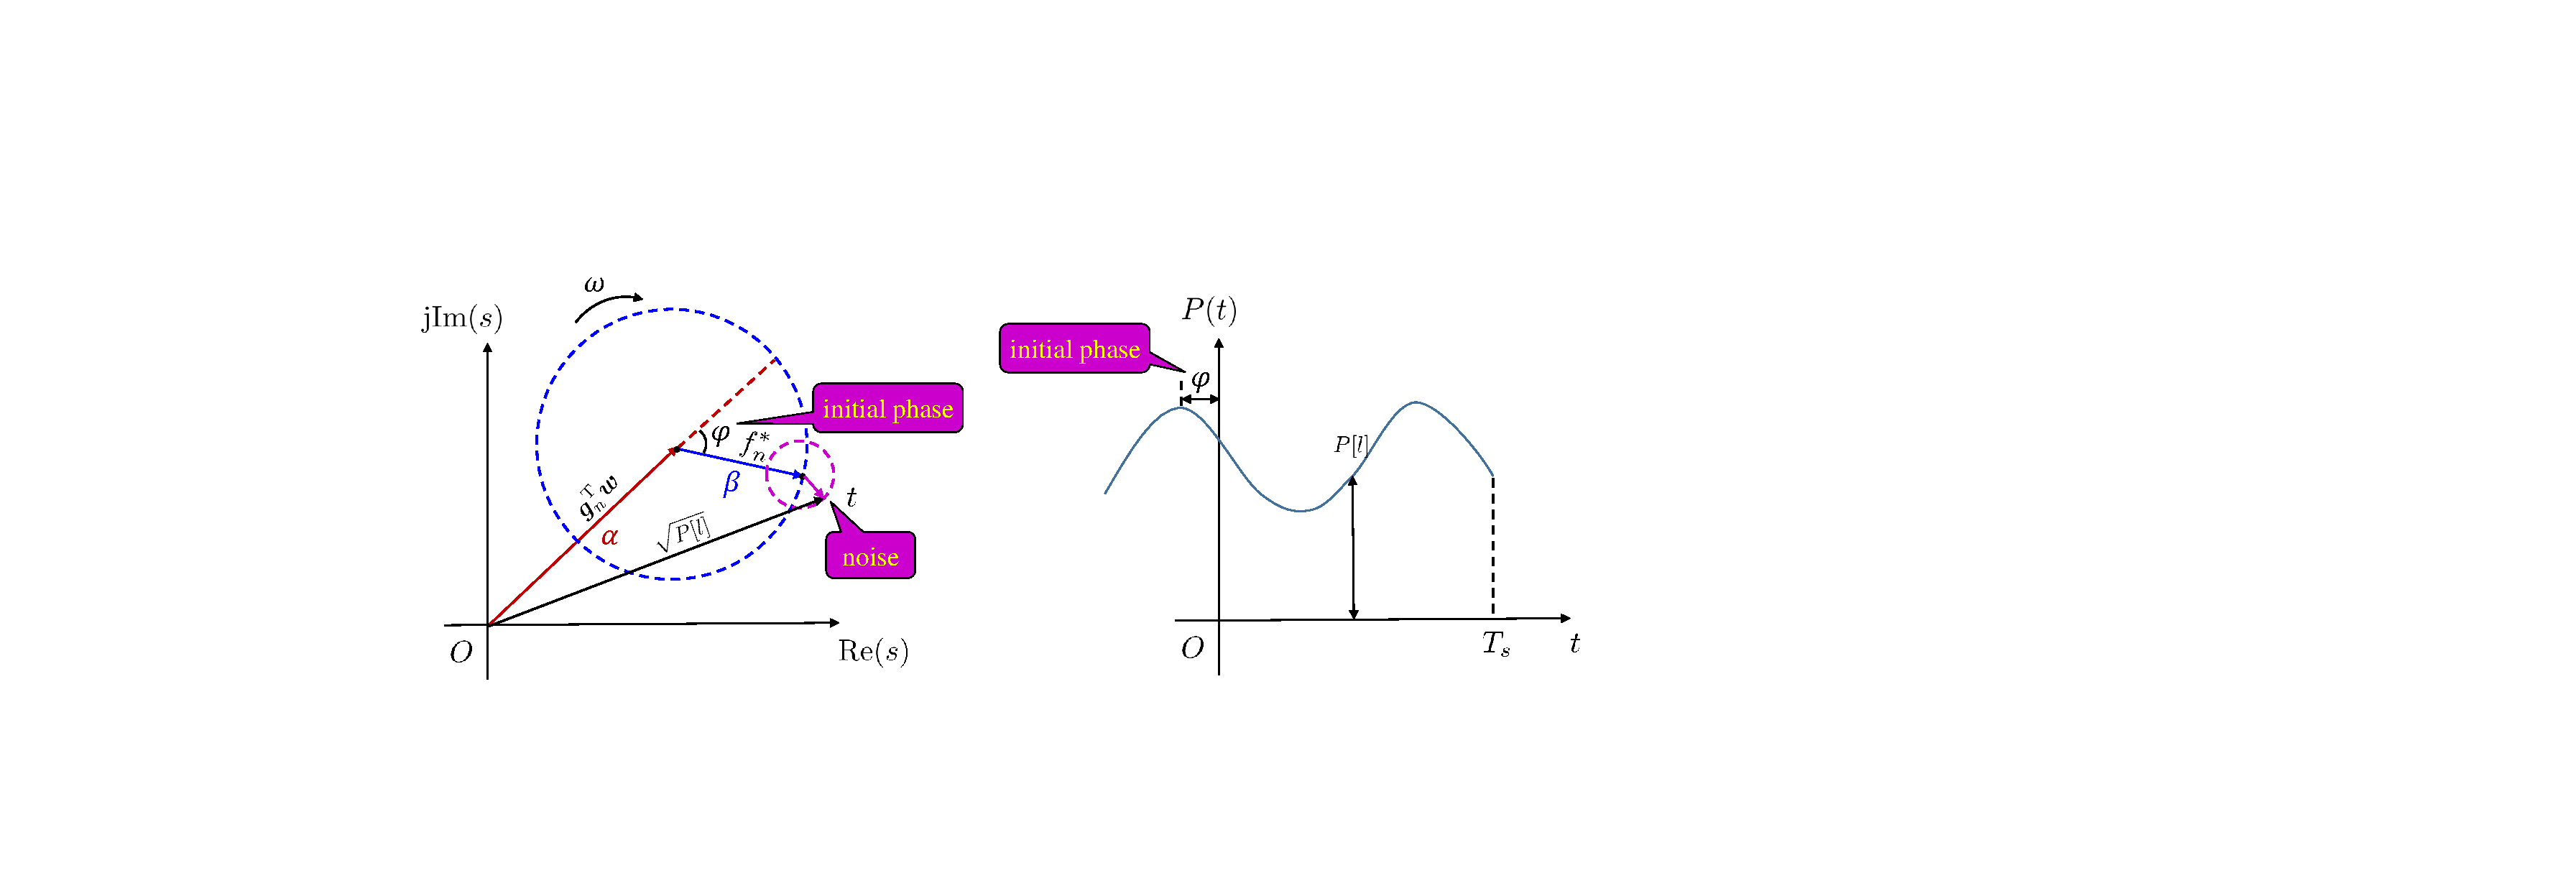
\includegraphics[width=\textwidth]{figures/phasor.pdf}
        \caption{Phasor representation of the \ac{IRF} on each RIS element. Red vector represents the complex BS-RIS signal ${\bm g}_n^T{\bm w}$; Blue vector represents the complex user-RIS signal $f_n^*w'$; $\alpha$ and $\beta$ denote the amplitude of these signals respectively. In our signaling method, the BS transmits a fixed symbol $s=1$, while the user transmits a rotating symbol $s'=e^{{\rm j}\psi(t)}$, causing the output of the power sensor $P(t)$ to vary in a waveform that is similar to a sine curve.}
        \label{fig:phasor}
    \end{figure}
    To further analyze the interference, we focus on the received IRF signal $P(t)$ of the $n$-th RIS element. 
    Note that the power of interference field measured at instant $t$, expressed by \eqref{eqn:power of interference}, exhibits a sinusoidal waveform in the time domain, as is shown in Fig.~\ref{fig:phasor}. 
    The initial phase ($t=0$) of this sinusoidal waveform is uniquely determined by $\varphi$.
    Thus, if we have access to the power received by the $n$-th element at successive instants $t_l$, it is possible to retrieve the phase difference $\varphi$. 
    However, according to \eqref{traditional beamforming}, it is the phase sum of the RIS-user channel and the BS-RIS channel, i.e., $\arg({\bm g}_n^{T}{\bm w})+\arg(f_n^*w')$, that determines the optimal phase-shift of the $n$-th element. Given the phase difference $\varphi = \arg\left(f_{n}^{*}w'\right)-\arg\left(\bm g_{n}^{T}\bm w\right)$, in order to acquire the phase sum, we only need to obtain one of the phases of these two channels to perform optimal RIS beamforming. Though generally it is difficult to obtain the BS-RIS channel and the RIS-user channel, since the BS and RIS are installed at fixed locations, it is reasonable to assume that the BS-RIS channel is much more stable and predictable, compared to the RIS-user counterpart. As a result, the phases of the BS-RIS link $\arg({\bm g}_n^{T}{\bm w})$ can be assumed to be known in our algorithms. Due to the stability of this channel, the phases are mainly determined by geometric parameters, i.e., the location of the BS and RIS. 


\section{Sensing RIS-Based Channel Estimation}
\label{Sensing RIS-Based Channel Estimation}
In this section, we will first briefly introduce the hardware architecture required for detecting the \ac{IRF} in Subsection~\ref{Hardware Architecture of Sensing RIS}. Then, the core concept of IRF channel estimation and beamforming procedures will be introduced in Subsection~\ref{IRF Channel Estimation and Beamforming}. Finally, Subsection~\ref{Pilot Overhead} will include the analysis on pilot overhead and computational complexity of our proposed IRF-based CSI acquisition methods. 

\subsection{Hardware Architecture of Sensing RIS} \label{Hardware Architecture of Sensing RIS}

    \begin{figure}[!t]
        \centering
        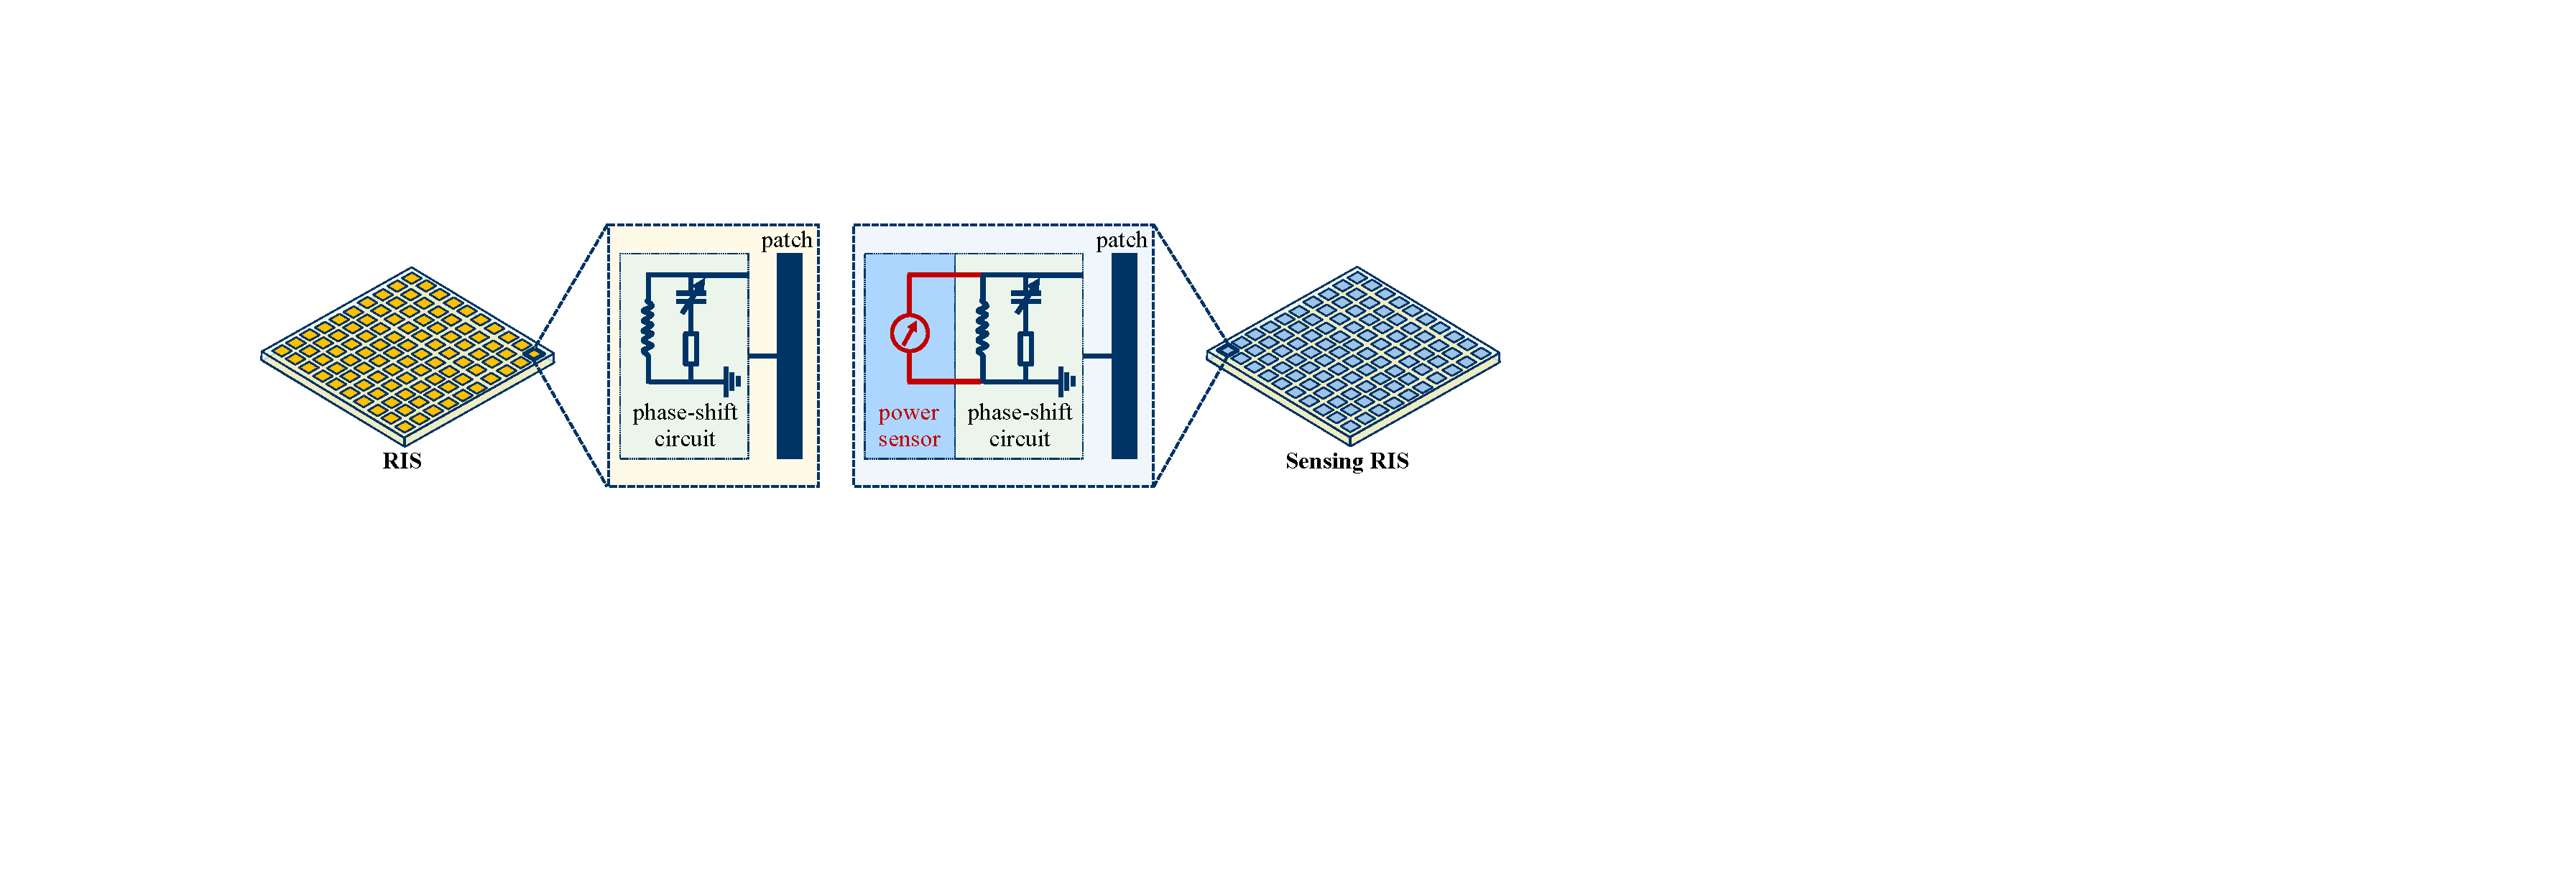
\includegraphics[width=\textwidth]{figures/hardware.pdf}
        \centerline{(a)~~~~~~~~~~~~~~~~~~~~~~~~~~~~~~~~~~~~~~~~~~~~~~~~~~~~(b)}
        \caption{Comparison of hardware architectures. (a) Traditional RIS. (b) Proposed sensing RIS.}
        \label{fig:hardware}
    \end{figure}
    
To obtain the amplitude of the induced \ac{IRF}, we propose a hardware architecture named sensing RIS.
In contrast to traditional RIS architecture shown in Fig.~\ref{fig:hardware}~(a), where each RIS element includes a phase-shift circuit and a patch antenna, each sensing RIS element additionally integrates a power sensor which is responsible for detecting the amplitude of the IRF \cite{ma2020smartsensing}, as shown in Fig.~\ref{fig:hardware}~(b).
Since all of the RIS elements can sense and adjust the phase independently from one another, low-cost microcontroller units (MCUs) can be attached locally to each RIS element to allow parallel computation of the optimal phases. 
However, for extremely large-scale RIS systems, sparse sensing and controlling may be preferred to reduce cost and hardware complexity. 

\subsection{IRF Channel Estimation and Beamforming} \label{IRF Channel Estimation and Beamforming}
    In this subsection, we will thoroughly introduce the IRF-based algorithms for adjusting the phases of the RIS elements. The \ac{IRF} channel estimation and beamforming procedure can be divided into three steps:
    \begin{enumerate}
        \item Simultaneous rotational signaling and power sensing; 
        \item Phase estimation based on power data;
        \item Integrate phase information and other CSI to perform beamforming. 
    \end{enumerate} 

    In step 1), three power signals are recorded: $P_{\alpha}(t)$, $P_{\beta}(t)$, and $P(t)$. The IRF appears during the third signal $P(t)$. 
    In order to create an IRF, simultaneous rotational signaling must be performed. 
    In fact, the signaling requirements can be realized by transmitting a symbol $s=1$ on the zeroth subcarrier at the BS, while transmitting a symbol $s'=1$ on the $k$-th subcarrier at the user. 
    As is mentioned above, if we denote the OFDM symbol period by $T_s$, then the equivalent IRF angular frequency $\omega$ is given by $\omega = 2\pi k /T_s$, which means the power signal exhibits exactly $k$ sine-shaped\footnote{The noiseless power signals are, in fact, strictly sinusoidal. } periods during an OFDM symbol. 
    For calculation simplicity, in this paper, we always assume $k=1$. 
    In fact, for multi-user MISO\footnote{In this paper, we assume that the user is equipped with a single antenna, but the number of antennas at BS is not restricted. Furthermore, for MIMO systems, since the user is equipped with multi-antennas, phase-tuning simply for constructive interference at the user is sub-optimal. Thus, IRF methods should be further improved to fully harness the multi-antenna space-multiplexing gains.} systems, different $k$ values can be assigned to different users in order to enable channel estimation and beamforming design for several users within a single OFDM symbol. 
    This can be done by Fourier analysis on the power signal $P(t)$ and extraction of phase angles for each user at distinct frequencies. 

    The second step 2) is called {\it phase estimation}. This step is designed to extract the phase difference $\varphi$ between the BS-RIS and RIS-user channel. 
    This is the key step of dimension-independent IRF channel estimation and beamforming, since this step can be done independently among all the RIS elements. 

    The third step 3) is to utilize the phase information provided by step 2) and calculate the near-optimal phase shifts for each RIS element in order to perform beamforming. The additional CSI refers to the phase information ${\rm arg}({\bm g}_n^T {\bm w})$. 

    Step 2) and step 3) are executed by processors, so we collect these two steps into pseudo codes shown in {\bf Algorithm~\ref{alg:IRF-Beamforming}}:
    \begin{algorithm}[H] 
        \caption{Near-optimal RIS Beamforming by IRF} \label{alg:IRF-Beamforming}
        \setstretch{1.35}
        \begin{algorithmic}[1]
            \REQUIRE Number of RIS elements $N$, IRF power signals detected on each RIS element $P_{\alpha}(t), P_{\beta}(t)$ and $P(t)$.
            \ENSURE RIS phase-shift matrix ${\bm \Theta}$.
            \FOR{$n=1,2,\cdots,N$}
                \STATE Estimate $\alpha$ and $\beta$ from $P_{\alpha}(t)$ and $P_{\beta}(t)$.
                \STATE Estimate phase difference $\varphi_n$ from $P(t)$, $\alpha$ and $\beta$. 
                \STATE Estimate $\psi_{n} = {\rm arg}(\bm g_{n}^{T}\bm w)$ from known locations of BS and RIS
                \STATE $\theta_n \leftarrow \exp(-{\rm j}(\varphi_n + 2\psi_n))$
            \ENDFOR
            \STATE ${\bm \Theta} \leftarrow \diag\left(\left[\theta_1, \theta_2, \cdots, \theta_N\right]^{T}\right)$
            \RETURN ${\bm \Theta}$
        \end{algorithmic}
    \end{algorithm}
    Note that in each iteration $n$ of {\bf Algorithm~\ref{alg:IRF-Beamforming}}, the data $P(t)$ is independent of other iterations. Thus, we can perform the calculations in parallel for each phase-shift $\theta_n$. For example, we can install an MCU for each of the elements on the RIS. Each MCU is only responsible for gathering the data from its own power sensor and adjusting the phase-shift of its own RIS element. Since all MCUs can work in parallel, the computational time is independent of the number of RIS elements, resulting in an $\mathcal{O}(1)$ time complexity. 

\subsection{Pilot Overhead and Computational Complexity}\label{Pilot Overhead}
    In our proposed IRF-based CSI acquisition method, the pilot overhead is fixed to $\mathcal{O}(1)$, which is independent of the RIS dimension $N$. 
    The reason is that, no matter how many RIS elements are employed, the IRF appears on them simultaneously. 
    Thus, both the channel estimation and beamforming can be fulfilled within only three pilot symbols, as is depicted in Fig.~\ref{fig:protocol}. 
    Thus, the pilot overhead is independent of the RIS dimension $N$. 
    To the best of our knowledge, this dimension-independent property is unprecedented, if we cannot endure the cost of attaching a dedicated RF chain to every RIS element. Some hybrid solutions do exist, such as connecting all the RIS elements to several RF chains with analog combiners\cite{alexandropoulos2021hybrid,alexandropoulos2020hardware} to enable explicit channel estimation at RIS. Unfortunately, the cost of analog combiners and RF chains are usually much higher than power sensors, which contradicts the original motivation of employing a cost-efficient RIS. 

    \begin{table}[!t]
        \centering
        \caption{Pilot Overhead Comparison of Different CSI Acquisition Methods}
        \label{tab:pilot overhead comp CE}
        \begin{tabular}{|c|c|c|}
            \hline 
            CSI acquisition method & Minimum pilot overhead & Applicable scenario \\ 
            \hline 
            Proposed IRF & 3 & Sensing-RIS \\ 
            \hline
            MVU\cite{jensen2020optimal}         & $NK+K$    & General \\
            \hline
            Multi-user\cite{wang2020channel}  & $K+N+\max \lbrace K-1, \lceil \frac{(K-1)N}{M} \rceil \rbrace$ & General \\
            \hline
            CS\cite{wei2021channel}          & $\mathcal{O}(KS\log N)$ & Sparse \\
            \hline 
            Two-timescale\cite{Huchen} & $\frac{2(N+1)}{\alpha} + K\lceil N/M\rceil +K$ & Slow variation \\
            \hline 
        \end{tabular}
    \end{table}

    Table~\ref{tab:pilot overhead comp CE} compares different CSI acquisition schemes. 

    The computational complexity of processing the obtained power signals depends on the hardware implementation. 
    The $\mathcal{O}(1)$ time complexity only holds when one MCU is installed for each RIS element. 
    If all the RIS elements are collectively controlled by one processor, the computational time would be $\mathcal{O}(N)$, but the pilot overhead still remains $\mathcal{O}(1)$. 
    These conclusions of complexity can be easily extended to multi-RIS schemes, where multiple RISs are employed to serve a single user at the same time. 
    The independent nature of IRF methods allows the RISs to work without the need to exchange data with the BS or other RISs. 
    This property makes it much easier to integrate a new RIS into an existing communication system, which greately enhances the extendibility of the system.

    


\section{Phase Estimation Algorithms}
In this section, three phase estimation algorithms will be proposed in Subsection~\ref{DFT method}, \ref{ML method}, and \ref{von Mises-EM method} respectively, which constitute the core of the \ac{IRF} channel estimation and beamforming algorithm.

\subsection{DFT method}  \label{DFT method}
    The key challenge of the IRF channel estimation and beamforming is the phase estimation step, i.e., how to obtain the phase difference $\varphi$. Since the interferential power $P(t)$ exhibits a sinusoidal waveform, Fourier transforms can be applied to extract its phase. Apply $L$-point \ac{DFT} to the discrete-time  observed sensor detection signals $P[0],\cdots ,P[L-1]$, and we have
    \begin{equation}
        \label{DFT}
        p[l']=\sum\nolimits_{l=0}^{L-1}P[l]e^{-{\rm j}\frac{2\pi}{L}ll'},\quad \forall l'\in \{L\}.
    \end{equation}
    Specifically, we have the complex amplitude of the first harmonics $p[1]$ as 
    \begin{equation}
        \label{DFT l=1}
        p[1]=\sum\nolimits_{l=0}^{L-1}A\left[\alpha^{2}+\beta^{2}+2\alpha\beta\cos\left(\frac{2\pi}{L}l+\varphi\right)\right]e^{-{\rm j}\frac{2\pi}{L}l}=LA\alpha\beta  e^{{\rm j}\varphi}.
    \end{equation}
    Then, the phase $\varphi$ can be estimated as
    \begin{equation}
        \label{LS estimate result}
        \hat{\varphi}=\arg\left(\frac{p[1]}{LA\alpha\beta}\right) = \arg\left(p[1]\right).
    \end{equation}
    Note that this DFT method simply ignores the non-Gaussian noise. For Gaussian noise, the DFT method is optimal. However, in fact, the noise in \eqref{eqn:power of interference} contains a squared term of a Gaussian noise, resulting the noise to be non-Gaussian. Thus, we further conceive an ML method, as described in the following Subsection~\ref{ML method}. 

\subsection{Newton-ML method}  \label{ML method}
    Suppose the noise field $v'(t)=v'_R(t) + {\rm j}v'_I(t)\sim \mathcal{CN}(0, \sigma_v^2)$, and the noise of the power sensor is $\zeta \sim \mathcal{N}(0, \sigma_{\zeta}^2)$. 
    Without loss of generality, we can assume that the sensor noise power $\sigma_{\zeta}^2$ is much weaker than the electromagnetic noise field $v'(t)$.
    Thus, we assume $\sigma_{\zeta}^2=0$ in the following discussion.  
    As a result, the distribution of $P(t) = A\left|E_{{\rm BB}, {\rm IRF}}(t)\right|^2$ is a non-central chi-squared distribution $\nc_{\chi_2^2}(A(\mu_{R}^2+\mu_{I}^2),  A\sigma_v^2/2)$ with degrees of freedom $k=2$, and mean values $\mu_{R}, \mu_{I}$ given by
    \begin{equation}
        \mu_{R} = \alpha + \beta \cos(\psi(t)+\varphi),\quad  \mu_{I}  = \beta \sin(\psi(t)+\varphi).
        \label{chi2 distribution mean values}
    \end{equation}
    Thus, according to \eqref{eqn:power of interference}, the output signal of the power sensor is given by 
    \begin{equation}
        P(t)  = A\left((v'_{R} + \mu_{R})^2 + (v'_{I} + \mu_{I})^2 \right)
        \label{eqn:sensor power}
    \end{equation}
    Let us define the noncentral parameter $\lambda(t)$ as
    \begin{equation}
        \lambda(t)  = A(\mu_{R}^2 + \mu_{I}^2) = A\left[\alpha^{2}+\beta^{2}+2\alpha\beta\cos\left(\psi(t)+\varphi\right)\right],
    \end{equation}
    then, according to the definition of the $\nc_{\chi_2^2}$, the p.d.f of $P(t)$ is given by the zeroth-order modified Bessel function of the first kind 
    \begin{equation}
        f_{P}(x) = \frac{1}{A\sigma_{v}^2} \exp\left(-\frac{x+\lambda(t)}{A\sigma_v^2}\right)I_{0}\left(\frac{\sqrt{\lambda(t) x}}{A\sigma_v^2/2}\right),\quad x \geq 0.
        \label{ML single observation}
    \end{equation}
    Then, the log likelihood function of $\varphi$ based on the observations $P[l]$ can be represented by
    \begin{equation}
        \mathcal{L}(P[0],\cdots,P[L-1] | \varphi) = \sum_{l=0}^{L-1}\left[-\frac{P[l] + \lambda_l}{A\sigma_v^2} + \log I_0\left(\frac{\sqrt{P[l] \lambda_l}}{A\sigma_v^2/2}\right)\right] - L\log(A\sigma_v^2),
        \label{ML likelihood}
    \end{equation}
    where $\lambda_l := \lambda(t_l)$, and the derivative of \eqref{ML likelihood} is 
    \begin{equation}
        \frac{\partial \mathcal{L}(P[0],\cdots,P[L-1] | \varphi)}{\partial \varphi} = \frac{2\alpha\beta}{\sigma_v^2}\sum_{l=0}^{L-1}\sin(\psi(t_l)+\varphi) \left[1 - R\left( \frac{\sqrt{P[l]\lambda_l}}{A\sigma_v^2/2} \right) \frac{\sqrt{P[l]}}{\sqrt{\lambda_l}}\right],
        \label{eqn:First Derivative Likelihood}
    \end{equation}
    where the function $R(z)$ is defined as $R(z) = I_1(z)/I_0(z)$. Since the derivative of the function $R(z)$ satisfies the property \cite{silverman1972special}
    \begin{equation}
        R'(z)=1-R^2(z)-\frac{1}{z}R(z),
        \label{eqn:R function derivative property}
    \end{equation}
    the second derivative of the likelihood function $\mathcal{L}$ can be expressed as
    \begin{equation}
        \begin{aligned}
        \frac{\partial^2 \mathcal{L}(P[0],\cdots,P[L-1] | \varphi)}{\partial \varphi^2}  = &  \frac{2\alpha\beta}{\sigma_v^2} \sum_{l=0}^{L-1}{\cos(\psi(t_l)+\varphi)}\left[1 - R\left(z_l\right) \frac{\sqrt{P[l]}}{\sqrt{\lambda_l}}\right] \\
        & +\frac{4\alpha^2\beta^2}{\sigma_v^4}\sum_{l=0}^{L-1}{\sin^2(\psi(t_l)+\varphi) \left(1-R^2(z_l) -\frac{2}{z_l}R(z_l)\right)\frac{P[l]}{\lambda_l} },\\
        \end{aligned}
        \label{Second Derivative Likelihood}
    \end{equation}
    where
    \begin{equation}
        z_l = \sqrt{P[l]\lambda(t_l)}/(A\sigma_v^2/2).
        \label{eqn:def z_l}
    \end{equation}
    Then, we can perform the Newton iteration to obtain $\hat{\varphi}$, by iteratively using the updating formula
    \begin{equation}
        \hat{\varphi}^{(k+1)} = \hat{\varphi}^{(k)} - \frac{\mathcal{L}'(\hat{\varphi}^{(k)})}{\mathcal{L}''(\hat{\varphi}^{(k)})},
        \label{eqn:Newton-ML renewal formula}
    \end{equation}
    where $\mathcal{L}'(\hat{\varphi}^{(k)})$ and $\mathcal{L}''(\hat{\varphi}^{(k)})$ are given by \eqref{eqn:First Derivative Likelihood} and \eqref{Second Derivative Likelihood} respectively. Note that during the calculation of \eqref{eqn:Newton-ML renewal formula}, $A, \sigma_v, \alpha, \beta$ and the received signal $P[l]$ are all assumed to be known. Thus, in fact,  \eqref{eqn:First Derivative Likelihood} and \eqref{Second Derivative Likelihood} are functions of a single variable $\varphi$. 

\subsection{von Mises-EM method}    \label{von Mises-EM method}
    The Newton-ML algorithm, if convergent, is asymptotically optimal \cite{casella2021statistical}. 
    However, the computation of the Newton-ML estimator is quite complicated due to intensive calculation of modified Bessel functions. 
    Now we introduce an iterative method for estimating $\varphi$ without any computation of such special functions.
    Our method is based on the von Mises distributions \cite{gatto2007generalized}.

    The von Mises-EM algorithm is based on the Bayesian inference of von Mises distributions \cite{mardia1976bayesian}. The von Mises distribution $\VM(\mu, \kappa)$ is a two-parameter distribution on $[0, 2\pi]$, with the probability density function given by 
    \begin{equation}
        p(\theta|\mu, \kappa) = \frac{\exp(\kappa \cos(\theta - \mu))}{2\pi I_0(\kappa)}, \quad 0\leq \theta \leq 2\pi,
    \end{equation}
    where $\mu \in [0,2\pi]$ and $\kappa >0$ being the cyclic location parameter and the concentration parameter. 
    Note that the von Mises distribution is a distribution on a circle, thus it acts as a perfect prior distribution of a phase estimation problem. 
    More fortunately, the von Mises distribution is also closely related to the complex Gaussian distribution, thus implying the possibility of designing an iterative EM algorithm \cite{casella2021statistical} based on the interactions between the von Mises distribution and the complex Gaussian noise distribution. The following two lemmas: {\bf Lemma \ref{lemma_1}} and {\bf Lemma \ref{lemma_2}} reveal these interactions. 
    \begin{lemma}[Bayesian estimation of von Mises distribution]\label{lemma_1} \mbox{}\par
        Let $\theta \sim \VM(\mu, \kappa)$, and $z|\theta \sim \CN(e^{{\rm j}\theta}, \sigma^2)$. Then the posterior distribution $\theta | z$ is also a von Mises distribution $\VM(\mu', \kappa')$ with parameters $\mu'$ and $\kappa'$ satisfying $\kappa' e^{{\rm j}\mu'} = \kappa e^{{\rm j}\mu} + 2z/\sigma^2$.
    \end{lemma}
        \begin{IEEEproof}
        See {\bf Appendix \ref{Proof of Lemma 1}}. 
    \end{IEEEproof}
    \begin{remark}
        From the above proof, we can also denote the von Mises distribution $\VM(\mu, \kappa)$ as $\VM(\kappa e^{{\rm j}\mu})$. This representation is more convenient when manipulating the posterior distribution of an $\VM$ distribution in Bayesian inference.
    \end{remark}

    \begin{lemma}[Noncentral $\CN$ posterior distribution on circle is $\VM$]\label{lemma_2} \mbox{}\par
        Suppose $z \sim \CN(z_0, \sigma^2)$, where $z_0 \in \mathbbm{C}$, and a positive radius $r>0$. Then the posterior distribution of angle $\theta= {\rm arg} (z)$, constrained on a circle $|z|=r$ obeys the von Mises distribution
        \begin{equation}
            p(\theta |\, |z|=r) \sim \VM\left({\rm arg}(z_0), \frac{r|z_0|}{\sigma^2/2}\right).
        \end{equation}
    \end{lemma}
    \begin{IEEEproof}
        Replacing $z$ by $r e^{{\rm j} \theta}$ give rise to the conclusion immediately. 
    \end{IEEEproof}
    Combining the results of {\bf Lemma \ref{lemma_1}} and {\bf Lemma \ref{lemma_2}}, we can then construct the EM algorithm for estimating $\varphi$. Since the output of the power sensors $P[l]$ does not contain phase information, we can treat the phases as latent variables. Let $s_l = \sqrt{P[l]/A}$ be the noisy estimation for $|\alpha + \beta e^{{\rm j} (\varphi + \psi_l)} + v_l|$, and $\theta_l$ be the latent variables $\arg (\alpha + \beta e^{{\rm j} (\varphi + \psi_l)} + v_l)$ that are not observable. 
    Since the noise $v_l \sim {\rm i.i.d.}\;\CN(0, \sigma_v^2)$, then from {\bf Lemma \ref{lemma_2}}, $\theta_l | s_l, \varphi \sim \VM(\arg(\alpha + \beta e^{{\rm j} (\varphi + \psi_l)}), s_l |\alpha + \beta e^{{\rm j} (\varphi + \psi_l)}|/(\sigma_v^2/2))$. Thus, we can infer the latent variables by ML estimation 
    \begin{equation}
        \hat{\theta}_{l, {\rm ML}} | s_l, \varphi = \arg(\alpha + \beta e^{{\rm j} (\varphi + \psi_l)}).
        \label{eqn:E-step}
    \end{equation}
    After inferring the latent variables $\hat{\theta}_{l, {\rm ML}}$, we can update the estimation of $\varphi$ using Bayesian rule in {\bf Lemma \ref{lemma_1}}
    \begin{equation}
        \varphi | s_l, \theta_l \sim \VM\left( \kappa e^{{\rm j} \mu} + \frac{\beta}{\sigma_v^2/2}\sum_{l=0}^{L-1}{\left(s_l e^{{\rm j}\theta_l}-\alpha\right)e^{-{\rm j} \psi_l}}\right),
        \label{eqn:M-step}
    \end{equation}
    where the coefficient $\beta/(\sigma_v^2/2)$ comes from scaling the phasor in Fig.~\ref{fig:phasor} by a factor $\beta^{-1}$ and applying {\bf Lemma \ref{lemma_1}}.
    Performing E-step with \eqref{eqn:E-step} and M-step with \eqref{eqn:M-step} alternately, then the estimation precision for $\varphi$ can be iteratively improved. Note that although the modified Bessel functions appear in the density function of von Mises distribution, the bother is avoided in the von Mises-EM algorithm. The pseudo code of von Mises-EM algorithm\footnote{We need the interferential parameters $\alpha$ and $\beta$, which are channel gains that can be directly measured within two time slots, without simultaneous signaling of the BS and the user. } is collected in {\bf Algorithm \ref{alg:VM-EM}}.

    \begin{algorithm}[htbp] 
        \caption{von Mises-EM phase estimation (VM-EM algorithm)} \label{alg:VM-EM}
        \setstretch{1.35}
        \begin{algorithmic}[1]
            \REQUIRE Incident wave intensity $\alpha$, $\beta$; sensor data $P[l]$; amplification factor $A$ and noise variance $\sigma_v^2$; predefined phase shifts $\psi_l=\omega t_l$.
            \ENSURE $\hat{\varphi}$
            \STATE $s_l \leftarrow \sqrt{P[l]/A}, \forall l=0,1,\cdots,L-1$
            \STATE $\hat{\varphi} \leftarrow \arg\{{\rm FFT}(P)[1]\}$
            \STATE $\kappa \leftarrow 1$
            \WHILE {$\hat{\varphi}$ not convergence}
                \STATE $\mu_l \leftarrow \alpha + \beta e^{{\rm j} (\hat{\varphi}+\psi_l)}, \forall l=0,1,\cdots,L-1$
                \STATE $w_l \leftarrow s_l e^{{\rm j} \arg(\mu_l)} - \alpha, \forall l=0,1,\cdots,L-1$
                \STATE $z_\varphi \leftarrow \kappa e^{{\rm j} \hat{\varphi}} + \beta \left( \sum_{l=0}^{L-1}{w_l e^{-{\rm j} \psi_l}}\right) / (\sigma_v^2/2)$
                \STATE $\hat{\varphi} \leftarrow \arg(z_\varphi)$
                \STATE $\kappa \leftarrow |z_\varphi|$
            \ENDWHILE
            \RETURN $\hat{\varphi}$
        \end{algorithmic}
    \end{algorithm}
    
\section{Performance Analysis}
\label{Performance Analysis}
    In this section, we will derive the \ac{CRLB} of the phase estimation problem. 
    Preliminaries about \ac{CRLB} will be introduced in Subsection~\ref{The CRLB}, and then precise CRLB and asymptotic CRLB will be derived in Subsection~\ref{Precise CRLB} and Subsection~\ref{Asymptotic CRLB}, respectively. Finally, the mathematical properties of the obtained \ac{CRLB} and error analysis will be provided in Subsection~\ref{Properties of the CRLB}. 

\subsection{The CRLB} \label{The CRLB}
    In the previous section, we have introduced three phase estimation methods. 
    A natural question is how accurate can these phase estimators be. 
    From \eqref{eqn:sensor power}, we can discover that the phase estimation is, in fact, a probabilistic parameter estimation problem, where the distributions of the observable variables are controlled by the parameter $\varphi$. 
    Thus, the ``best'' mean squared error of any unbiased estimator is lower-bounded by the CRLB \cite{casella2021statistical} 
    \begin{equation}
        \mathbb{E}\left(\hat{\varphi}-\varphi\right)^2 \geq {\rm CRLB}(\varphi) = -\frac{1}{\mathbb{E}_{x\sim p_\varphi}\left[\frac{\partial^2}{\partial\varphi^2}\log p_{\varphi}(x)\right]},
        \label{eqn:CRLB definition}
    \end{equation}
    where $p_{\varphi}(x)$ is the distribution of $x$ when the parameter is $\varphi$, and in this paper $p_{\varphi}(x)$ obeys a non-central chi-squared distribution. 

    The evaluation of CRLB in non-coherent parameter estimation was first formulated in \cite{jiang2016cramer}, where the authors introduced Gaussian approximation in order to obtain a simple closed-form CRLB expression. Unfortunately, this approximation only holds for very large non-centrality parameter $\lambda$, i.e., large interferential SNR $\gamma=\lambda/A\sigma_v^2$. Thus, precise CRLB analysis is required in our \ac{IRF} methods. However, without Gaussian approximation techniques, fatal complexity about Bessel functions will occur, making the analysis nearly intractable. 

    To overcome this difficulty, we first perform precise analysis, and then approximated asymptotic analysis. The difficulty of manipulating Bessel functions is conquered by asymptotic expansion techniques \cite{silverman1972special}. Satisfactory asymtotic results are acquired in the absence of precise closed-form expression of CRLB. These results will be introduced in the following subsection.  
    %In the following two subsections, {\bf Theorem \ref{thm:precise CRLB}} reveals  
    
\subsection{Precise CRLB} \label{Precise CRLB}
    \begin{theorem}[Non-central Chi-Squared CRLB] \label{thm:precise CRLB}\mbox{}\par
        Suppose the probabilistic model is specified by \eqref{eqn:sensor power}, where $L$ observations are obtained at instants $t_l, \forall l\in P[0],\cdots,P[L-1]$. Then the CRLB of this $L$-point phase estimation problem is given by
        \begin{equation}
            \frac{1}{{\rm CRLB}(\varphi)} = K^2(\bar{\gamma})^2 \sum_{l=0}^{L-1}\sin^2(\psi_l+\varphi)\left(1/\gamma_l-g(\gamma_l)\right),
            \label{eqn:precise_CRLB}
        \end{equation}
        where $K=2\alpha\beta/(\alpha^2+\beta^2)$, $a=A\sigma_v^2$, $\gamma_l=\lambda_l/a=\left(\alpha^2+\beta^2+2\alpha\beta \cos(\psi_l+\varphi)\right)/\sigma_v^2$, and $\bar{\gamma}$ is the arithmetic mean of all the $\gamma_l, 0\leq l<L$. The function $g(\gamma)$ is defined as 
        \begin{equation}
            \begin{aligned}
                g(\gamma) &= \mathbb{E}_{x\sim \nc_{\chi_2^2}(\lambda, a)}\left[\left(1-R^2\left(\frac{\sqrt{\lambda x}}{a/2}\right)\right)\frac{x}{\lambda}\right] \\
                & = \int_{0}^{+\infty}\gamma t \, {\rm exp}(-\gamma(1+t))\, I_0\left(2\gamma\sqrt{t}\right)\,\left(1-R^2\left(2\gamma\sqrt{t}\right)\right){\rm d}t.
            \end{aligned}
            \label{eqn:precise_g_function}
        \end{equation}
        Furthermore, $\bar{\gamma}$ is determined only by physical signal intensity
        \begin{equation}
            \bar{\gamma} = \frac{1}{L}\sum_{l=0}^{L-1}{\gamma_l} = \frac{\alpha^2+\beta^2}{\sigma_v^2}.
        \end{equation}
        The function $R(\cdot)$ is defined the same as in \eqref{eqn:R function derivative property}. Also note that the CRLB of the phase estimation problem is completely determined by the two parameters $K$ and $\bar{\gamma}$. 
    \end{theorem}
    \begin{IEEEproof}
        See {\bf Appendix \ref{appendix:proof of theorem1}}. 
    \end{IEEEproof}

    In analogy to optics, the parameter $K$ in \eqref{eqn:precise_CRLB} is called the interferential contrast. And the parameter $\bar{\gamma}$ is the average interferential SNR, since $\gamma_l=\lambda_l/a = (\mu_{R}^2+\mu_{I}^2)/\sigma_v^2$ is the ratio of the noiseless power signal and the noise power. Thus, the CRLB expression \eqref{eqn:precise_CRLB} has strong physical meanings. However, this precise CRLB expression is difficult to evaluate due to the sophisticated evaluation of integral in \eqref{eqn:precise_g_function}, hence it is more feasible to obtain a simpler approximated CRLB with closed-form expression. 

\subsection{Asymptotic CRLB}    \label{Asymptotic CRLB}
    \begin{theorem}[Asymptotic Evaluation of Noncentral Chi-Squared CRLB] \label{thm:asymptotic CRLB} \mbox{}\par
        Suppose the probabilistic model is specified by \eqref{eqn:sensor power}. Then the approximated CRLB of this $L$-point phase estimation problem is given by 
        \begin{equation}
            \frac{1}{{\rm CRLB}(\varphi)}\approx K^2(\bar{\gamma})^2 \sum_{l=0}^{L-1}\sin^2(\psi_l+\varphi)(1/\gamma_l-\hat{g}(\gamma_l))^{+},
            \label{eqn:asymptotic CRLB}
        \end{equation}
        where $(x)^{+}$ represents ${x{\mathbbm{1}}_{\{x\geq 0\}}}$, and the definition of parameters are the same as in {\bf Theorem \ref{thm:precise CRLB}}. The asymptotic approximation function $\hat{g}(\gamma)$ is defined as 
        \begin{equation}
            \hat{g}(\gamma) = \frac{1}{4} \sqrt{\frac{\pi}{\gamma}}e^{-\gamma/2}\left((1+1/\gamma)I_0(\gamma/2) + I_1(\gamma/2)\right).
            \label{eqn:definition g function}
        \end{equation}
    \end{theorem}
    \begin{IEEEproof}
        See {\bf Appendix \ref{Proof of Theorem 2}}. 
    \end{IEEEproof}
    \begin{remark}
        The asymptotic result of CRLB still relies only on two parameters $K$ and $\bar{\gamma}$. But the calculation is much simpler compared to the precise CRLB. 
    \end{remark}

\subsection{Properties of the CRLB} \label{Properties of the CRLB}
    From the above analysis, we have obtained the precise and asymptotic versions of CRLB expressions. Furthermore, from these expressions, we can observe two properties of the phase estimation problem:
    \begin{enumerate}
        \item The CRLB relies almost only on the physical parameters $K$ and $\bar{\gamma}$.
        \item The CRLB is insensitive to the value $\varphi$.
    \end{enumerate}
    The first point can be concluded from the expressions, and the second point comes from the symmetry of the $\sin^2(\cdot)$ function when $L$ is large enough. Thus, we can plot $1/{\rm CRLB}(\varphi)$ as a two-variable function (see Fig.~\ref{fig:CRLB two variable}). 
    \begin{figure}[!t]
        \centering
        \myincludegraphics{data/CRLB.pdf}
        \caption{Precise $1/{\rm CRLB}(\varphi)$ as a two-variable function of $K$ and $\bar{\gamma}$, calculated from \eqref{eqn:precise_CRLB}. The larger the value of reciprocal CRLB, the more precise an unbiased estimator can be. }
        \label{fig:CRLB two variable}
    \end{figure}
    The best prediction accuracy occurs when $\lvert K \rvert = 1$, i.e., the RIS-received signal from BS is as strong as that from the user. 
    Also, the larger value of the average interferential SNR $\bar{\gamma}$ also contributes to more accurate phase estimation. 

    However, error analysis is vital to any kind of approximated analysis. Fortunately, our asymptotic expansion technique allows very good approximation, which is verified in the following {\bf Theorem 3}. 

    \begin{theorem}[CRLB Approximation by Asymptotic Expansion is Asymptotically Optimal] \label{thm_error_analysis}
        The relative error $r$ of $1/\gamma - \hat{g}(\gamma)$, as an approximation of $1/\gamma - g(\gamma)$, decreases at a rate that is inverse proportional to the interferential SNR $\gamma$, i.e.,
        \begin{equation}
            r=\frac{\left|\hat{g}(\gamma)-g(\gamma)\right|}{1/\gamma - g(\gamma)} = \mathcal{O}\left(\frac{1}{\gamma}\right).
        \end{equation}
    \end{theorem}
    \begin{IEEEproof}
        See {\bf Appendix \ref{Proof of Theorem 3}}. 
    \end{IEEEproof}
    \begin{remark}
        From {\bf Theorem \ref{thm_error_analysis}} we can also conclude that the relative error of \eqref{eqn:asymptotic CRLB} is also of order $\mathcal{O}(1/\bar{\gamma})$ for any $K>0$. 
    \end{remark}


\section{Simulation Results}
\label{Simulation Results}
In this section, we will present our simulation results. In Subsection \ref{Phase Estimation Algorithms}, we will show the performance comparison of the phase estimation algorithms. In Subsection \ref{Achievable Spectral Efficiency under IRF}, we will show the achievable rate comparison of our \ac{IRF} method and other RIS-aided channel estimation and beamforming algorithms. 

\subsection{Phase Estimation Algorithms} \label{Phase Estimation Algorithms}
    In Section~\ref{Sensing RIS-Based Channel Estimation}, we have already introduced three phase estimation algorithms: DFT, Newton-ML and VM-EM. Now we compare the performance of these algorithms together with the CRLB which has been derived in Section~\ref{Performance Analysis}. 
    \begin{figure}[!t]
        \centering
        \myincludegraphics{data/pe_K.pdf}
        \caption{Performance comparison of phase estimation algorithms. $x$-axis represents the interferential contrast $K$; $y$-axis represents the MSE of the estimators. The VM-EM algorithm outperforms naive DFT by at least $1\,{\rm dB}$ in high-$K$ regions. }
        \label{fig:phase estimation_K}
    \end{figure}
    % Insert the comparison figure w.r.t \bar{\gamma}.
    \begin{figure}[!t]
        \centering
        \myincludegraphics{data/pe_gamma.pdf}
        \caption{Performance comparison of phase estimation algorithms. $x$-axis represents the average interferential SNR $\bar{\gamma}$; $y$-axis represents the MSE of the estimators. The interferential contrast $K=0.6$. }
        \label{fig:phase estimation_gamma}
    \end{figure}
    In all the simulations for phase estimation algorithms, the amplification factor $A$ is fixed to be $1$, the number of power samples\footnote{In practical OFDM systems, the number of signal samples within the duration of an OFDM symbol is usually $\sim 2048$. Considering that the power sensor is usually slower than the baseband ADC, it is reasonable to assume a 32-times slower sampling rate of the power sensor. Thus, $L=64$ is a reasonable number of acquired power samples during one time slot.} is fixed to $L=2^6=64$, and $\sigma_\zeta=0.05$; 
    The interferential SNR $\bar{\gamma}=20$ in Fig.~\ref{fig:phase estimation_K}. 
    The CRLB and CRLB-approx curves are calculated from \eqref{eqn:precise_CRLB} and \eqref{eqn:asymptotic CRLB}, respectively. 
    For Newton-ML algorithm, the Newton iteration is performed 4 times according to \eqref{eqn:Newton-ML renewal formula}. 
    For VM-EM algorithm, the iteration number is also fixed to 4. The true value of random variable $\varphi$ under estimation is drawn from a uniform distribution on $[0,2\pi]$. 
    In the simulations in Fig.~\ref{fig:phase estimation_gamma}, all the simulation parameters, except for $K$ and $\bar{\gamma}$, are the same with Fig.~\ref{fig:phase estimation_K}.

    From Fig.~\ref{fig:phase estimation_K} and Fig.~\ref{fig:phase estimation_gamma} we discover that the VM-EM algorithm has comparable performance with the Newton-ML algorithm, but the computational cost is significantly lower, since {\bf Algorithm \ref{alg:VM-EM}} does not require the evaluation of the complicated modified Bessel functions. 
    Both the Newton-ML and VM-EM algorithms are close to CRLB, and both of them outperform the simple DFT algorithm\footnote{The DFT estimator in Fig.~\ref{fig:phase estimation_gamma} exhibits a near-constant performance gap towards the CRLB in the high-SNR region, while the Newton-ML and VM-EM estimators seem to bridge this gap and finally approaches the CRLB as $\bar{\gamma}\to\infty$.}. 
    The CRLB approximation is also satisfactory under a wide range of $K$ and $\bar{\gamma}$. 

\subsection{Achievable Spectral Efficiency under IRF} \label{Achievable Spectral Efficiency under IRF}
    \begin{figure}[!t]
        \centering
        \myincludegraphics{data/rate.pdf}
        \caption{Performance curve of the achievable spectral efficiency against the BS transmitted power $P_{\rm max}$.}
        \label{fig:rate}
    \end{figure}
    All our simulation data are acquired under $P_{\rm max}'=300 \,{\rm mW}$, $n_0=-174\,{\rm dBm/Hz}$, subcarrier bandwidth ${\rm BW} = 180\,{\rm kHz}$, thermal noise at the receiver $\sigma^2 = {\rm BW}\times n_0$, $\sigma_v^2=100\,{\rm MHz}\times n_0$, and the BS-RIS and RIS-user channels are all assumed to be Rayleigh fading with 1 LOS path and 4 NLOS paths. The LOS path has, on average, $\kappa$ times more energy than the NLOS paths together, and $\kappa=2$. Both the BS and the RIS are equipped with $\lambda/2$-spaced uniform planar arrays (UPAs), while the user has a single antenna. 
    The BS is located at a distance from the RIS that is drawn from a uniform distribution between $20\,{\rm m}$ and $100\,{\rm m}$, and the angle of the BS is uniformly distributed. The user appears uniformly from $10\,{\rm m}$ to $100\,{\rm m}$, and the angle distribution of the user is also uniform. The size of the RIS is set to be $40\times 30$, and that of the BS antenna is $4\times 2$. For IRF methods, 3 pilots are used for CSI acquisition. 
    However, for LS-CE methods, the number of pilots is $N=40\times 30$. 

    We compare our proposed \ac{IRF} channel estimation and beamforming method with classical LS-CE algorithm and other idealized settings in Fig.~\ref{fig:rate}. The black dashed line ``Oracle'' assumes perfectly-known CSI, thus perfect iterative beamforming can be performed. In the LS-CE method, we first utilize \eqref{eqn:LS-CE} to obtain estimates for the cascaded channel \cite{kundu2021channel,wei2021channel}, and then perform iterative RIS beamforming based on the estimated channel. In addition, we also consider the randomly-phased RIS scheme as a benchmark.  

    Fig.~\ref{fig:rate} shows the performance curve of the achievable spectral efficiency against the BS transmitted power. From this figure, we can conclude that the proposed IRF method with VM-EM phase estimation is nearly optimal, under extremely low pilot overhead. The proposed IRF method is even close to the oracle scheme, and has satisfactory performance among a wide range of the BS transmitted power. 



\section{Conclusion}
\label{Conclusion}
    In this paper, we introduced a dimension-independent CSI acquisition method for sensing RIS-assisted MISO wireless communication systems. 
    Combined with our proposed VM-EM phase estimation algorithm, the pilot overhead of our CSI acquisition method is made independent of the number of RIS elements with low computational cost, enabling the implementation of extremely large-scale RISs to achieve significant beamforming gain. 
    Both CRLB analysis and simulation results verified the near-optimality of our VM-EM algorithm. 
    Furthermore, due to the independent property of our \ac{IRF}-based CSI acquisition method, the near-field effect cannot corrupt the precision of the CSI. 
    Also due to the simultaneous signaling protocol, the “multiplicative fading” effect of RIS \cite{zhang2021active,liu2021active} during channel estimation is automatically avoided. 
    Thus, the \ac{IRF} method has a promising future in high-frequency large-scale systems. 
    
    For future work, the spatial interferential fringes on the sensing RIS may be exploited to recover the CSI at higher precision, and the data obtained by the power sensors may be utilized to perform joint channel estimation and beamforming together with traditional methods. 
    In addition, different interferential frequencies can be assigned to different users to perform multi-user CSI acquisition within a single time slot, but the waveforms should be re-designed to avoid interference among users. 
    Furthermore, when equipped with a sensing RIS, traditional MIMO systems can also benefit from the additional CSI provided by the phase estimation methods of IRF.  
% This is the end of the "Conclusion" part. 

\appendices
% Non-central Chi-Squared distribution. 
\section{Proof of \textbf{Lemma 1}}
\label{Proof of Lemma 1}
        Denote $z=z_r + {\rm j} z_i$, then the posterior density $p(\theta | z) \propto p(\theta)p(z|\theta)$ can be expressed as
        \begin{equation}
            \begin{aligned}
                p(\theta|z) & \propto \exp(\kappa \cos(\theta - \mu))\exp\left(-\frac{1}{\sigma^2}\left(\left(z_r - \cos\theta\right)^2 + \left(z_i - \sin\theta\right)^2\right)\right) \\
                & \propto \exp\left( \kappa \cos(\theta - \mu) + \frac{2}{\sigma^2}(z_r \cos\theta + z_i\sin\theta) \right) \\
                & \propto \exp\left( \re\left[ e^{{\rm j} \theta}\left(\kappa e^{-{\rm j}\mu} + \frac{1}{\sigma^2/2} z^*\right)\right] \right).
            \end{aligned}
        \end{equation}
        Since the density of von Mises distribution $\VM(\mu, \kappa)$ can also be expressed as $p(\theta) \propto \exp\left( \re\left[ e^{{\rm j} \theta}(\kappa e^{{\rm j} \mu})^* \right] \right)$, we can also parameterize the von Mises distribution by a single complex parameter $\kappa e^{{\rm j}\mu}$. Thus, the above $p(\theta|z)$ is a von Mises density with parameter $\kappa'e^{{\rm j}\mu'}$, satisfying $\kappa' e^{{\rm j}\mu'} = \kappa e^{{\rm j}\mu} +2z/\sigma^2$. This completes the proof.


\section{Proof of \textbf{Theorem 1}}\label{appendix:proof of theorem1}
    According to the definition of CRLB \eqref{eqn:CRLB definition}, taking the negative expectation of \eqref{Second Derivative Likelihood} yields the reciprocal CRLB of the estimators for $\varphi$. Note that in \eqref{Second Derivative Likelihood}, there are three types of expectations to be evaluated: $\mathbb{E}\left[P[l]\right]$, $\mathbb{E}\left[R(z_l)\sqrt{P[l]}\right]$, and $\mathbb{E}\left[(1-R^2(z_l))P[l]\right]$. The expectation of $P[l]$ can be directly evaluated from \eqref{eqn:sensor power} by the linearity of the expectation operation:
    \begin{equation}
        \mathbb{E}\left[P[l]\right] = A\sigma_v^2 + \lambda_l.
        \label{eqn:expectation of P_l}
    \end{equation}
    The expectation $\mathbb{E}\left[R(z_l) \sqrt{P[l]}\right]$ can be evaluated by calculating the derivative w.r.t $\lambda_l$ on both sides of the identity $\mathbb{E}_{\lambda_l, A\sigma_v^2}[e^{\lambda_l/(A\sigma_v^2)}]=e^{\lambda_l/(A\sigma_v^2)}$:
    \begin{equation}
        \begin{aligned}
            \mathbb{E}\left[R(z_l) \sqrt{P[l]}\right] & = e^{-\lambda_l/(A\sigma_v^2)}\int_{0}^{+\infty}{\frac{1}{A\sigma_v^2}\exp\left(-\frac{x}{A\sigma_v^2}\right)I_1\left(\frac{\sqrt{\lambda_l x}}{A\sigma_v^2/2}\right)\sqrt{x}{\rm d}x} \\
            & = e^{-\lambda_l/(A\sigma_v^2)} A\sigma_v^2 \sqrt{\lambda_l} \frac{\partial}{\partial\lambda_l} \int_{0}^{+\infty}{\frac{1}{A\sigma_v^2}\exp\left(-\frac{x}{A\sigma_v^2}\right)I_0\left(\frac{\sqrt{\lambda_l x}}{A\sigma_v^2/2}\right) {\rm d}x}\\
            & = \sqrt{\lambda_l}.\\
        \end{aligned}
        \label{eqn:expectation_second_kind_1}
    \end{equation}
    Note that, because of the definition of $z_l$ \eqref{eqn:def z_l}, the expectation $\mathbb{E}\left[R(z_l)P[l]/z_l\right]$ is, intrinsically, of the same form as the expectation $\mathbb{E}\left[R(z_l) \sqrt{P[l]}\right]$. Thus, the expectation result is
    \begin{equation}
        \mathbb{E}\left[\frac{R(z_l)}{z_l} P[l]\right] = \frac{A\sigma_v^2}{2}.
        \label{eqn:expectation_second_kind_2}
    \end{equation}
    The third kind of expectation $\mathbb{E}\left[(1-R^2(z_l))\frac{P[l]}{\lambda_l}\right]$ is the trickiest to calculate, since it has no closed-form expression. So we define the two-variable $g$ function to be 
    \begin{equation}
        g(\lambda_l, a) = \mathbb{E}\left[(1-R^2(z_l))\frac{P[l]}{\lambda_l}\right].
        \label{eqn:two-variable g function}
    \end{equation}
    It is not trivial to observe that the two-variable function $g(\lambda_l, a)$ is, in fact, a single-variable function $g(\gamma_l)$, with $\gamma_l=\lambda_l/a$. Let $x=\lambda_l t$, and write down the integral expression of \eqref{eqn:two-variable g function}, we obtain 
    \begin{equation}
        \begin{aligned}
        g(\lambda_l, a) & = \int_{0}^{+\infty} t(1-R^2(2\gamma_l\sqrt{t})) \frac{\lambda_l}{a} \exp\left(\frac{\lambda_l + \lambda_l t}{a}\right) I_0\left(2\gamma_l\sqrt{t}\right){\rm d}t \\
        & = \int_{0}^{+\infty}\gamma_l t \, \exp(-\gamma_l(1+t))\, I_0\left(2\gamma_l\sqrt{t}\right)\,\left(1-R^2\left(2\gamma_l\sqrt{t}\right)\right){\rm d}t \\
        & = g(\gamma_l).
        \end{aligned}
        \label{eqn:proof precise g function}
    \end{equation}
    
    Combining the above equations of expectations \eqref{eqn:expectation of P_l}, \eqref{eqn:expectation_second_kind_1}, \eqref{eqn:expectation_second_kind_2} and \eqref{eqn:proof precise g function}, we obtain
    \begin{equation}
        \begin{aligned}
        \frac{1}{{\rm CRLB}(\varphi)} %& = -\mathbb{E}\left[\frac{\partial^2\mathcal{L}}{\partial\varphi^2}\right] \\
        & \overset{(a)}{=}  -\frac{4\alpha^2\beta^2}{\sigma_v^4}\sum_{l=0}^{L-1}{ \sin^2(\psi(t_l)+\varphi) \left(\mathbb{E}\left[(1-R^2(z_l))\frac{P[l]}{\lambda_l}\right] - \frac{a}{\lambda_l}\right) } \\
        & \overset{(b)}{=} \frac{4\alpha^2\beta^2}{\sigma_v^4}\sum_{l=0}^{L-1}{ \sin^2(\psi(t_l)+\varphi) \left(\frac{a}{\lambda_l}-g(\lambda_l/a)\right)},
        \end{aligned}
        \label{eqn:CRLB}
    \end{equation}
    where step $(a)$ comes from substituting these three types of expectation into \eqref{Second Derivative Likelihood}, and step $(b)$ comes from replacing the trickiest expectation by the definition of the function $g(\cdot)$ in \eqref{eqn:precise_g_function}.  
    
    Note that the precise value of CRLB can be determined by the precise single-variable $g$ function \eqref{eqn:precise_g_function}, whose variable $\gamma_l = \lambda_l / a$ is the interferential SNR. After further derivations, it can be observed from the expressions that the CRLB only relies on two intrinsic physical parameters: the interferential SNR $\gamma_l$, and the interferential contrast $K$ \cite{louradour1993interference}, which coincides with the physical intuition. Imitating the notations in optics, we define the parameter $K$ to be  
    \begin{equation}
        K = \frac{I_M - I_m}{I_M + I_m} = \frac{2\alpha\beta}{\alpha^2+\beta^2},
    \end{equation}
    and $K$ automatically satisfies $-1\leq K\leq 1$. Define the average interferential SNR $\bar{\gamma}$ to be the arithmetic average of $\gamma_l, 0\leq l < L$:
    \begin{equation}
        \bar{\gamma} = \frac{1}{L}\sum_{l=0}^{L-1}{\gamma_l} = \frac{\alpha^2+\beta^2}{\sigma_v^2}.
    \end{equation}
    Thus, the CRLB can be expressed as 
    \begin{equation}
        \frac{1}{{\rm CRLB}(\varphi)} = K^2(\bar{\gamma})^2 \sum_{l=0}^{L-1}{ \sin^2(\psi_l+\varphi) \left(1/\gamma_l-g(\gamma_l)\right) }
    \end{equation}
    where the values $\gamma_l=\bar{\gamma}\left(1+K\cos(\psi_l+\varphi)\right)$ are jointly determined by both the average interferential SNR $\bar{\gamma}$ and the interferential contrast $K$. This completes the proof.

\section{Proof of \textbf{Theorem 2}}
\label{Proof of Theorem 2}
    Since the precise expression of $g(\gamma)$ in \eqref{eqn:precise_g_function} is difficult to calculate, we evaluate it approximately by utilizing the asymptotic expansion $x(1-R^2(2\sqrt{x})) \approx \sqrt{x}/2$ \cite{silverman1972special}. According to the definition, evaluating $g(\gamma)$ is the same as evaluating $\mathbb{E}[(1-R^2(z_l))P[l]/\lambda_l]$. 
    % Thus, by substituting $x=\lambda_lP[l]/a^2$ into the asymptotic expansion formula, we can further simplify the integrand of the expectation to be 
    % \begin{equation}
    %     \begin{aligned}
    %         \mathbb{E}\left[(1-R^2(z_l))\frac{P[l]}{\lambda_l}\right] & \approx g(\lambda_l, a) \\ 
    %         & \triangleq  \frac{1}{4}\sqrt{\frac{\pi a}{\lambda_l^3}}e^{-\lambda_l/(2a)}\left((a+\lambda_l)I_0(\lambda_l/(2a))+\lambda_l I_1(\lambda_l/(2a))\right),
    %     \end{aligned}
    %     \label{eqn:trickiest_expectation}
    % \end{equation}
    % where $a=A\sigma_v^2 \ll \lambda_l$, $h(\lambda_l, a)$ is a two-variable function\footnote{In fact, the two-variable function $g(\lambda, a)$ can be further simplified into a single-variable function $g(\cdot). $}, and $I_\nu$ is the $\nu$-th order  modified Bessel function of the first kind. For detailed proof of the calculation process and error analysis of \eqref{eqn:trickiest_expectation}, please refer to {\bf Appendix B}. 


    In order to evaluate the expectation $\mathbb{E}[(1-R^2(z_l))P[l]/\lambda_l]$, we first introduce some preliminaries about the noncentral chi distribution $\nc_{\chi_k}(\lambda)$ with noncentrality parameter $\lambda>0$. The distribution $\nc_{\chi_k}(\lambda)$ is the law of the length (2-norm) of a $k$-dimensional standard normal distribution $\mathcal{N}({\bm \mu}, {\bm I}_k)$, with $\lambda = \Vert {\bm \mu} \Vert_2$. Specifically, we are interested in the case where $k=2$, since this is the case of the 2-dimensional complex plane. For  $k=2$, let $Y \sim \nc_{\chi_2}(m)$, then we have \cite{park1961moments}
    \begin{equation}
        \mathbb{E}\left[Y\right] = \sqrt{\frac{\pi}{2}}L_{1/2}(-m^2/2),
        \label{eqn:noncentral chi mean}
    \end{equation}
    where $L_{1/2}$ denotes the generalized Laguerre function  of order $1/2$. The function $L_{1/2}(x)$ has explicit expression 
    \begin{equation}
        L_{1/2}(x) = e^{x/2}\left[(1-x)I_0\left(-\frac{x}{2}\right)-xI_1\left(-\frac{x}{2}\right) \right].
        \label{eqn:Laguerre half order}
    \end{equation}
    Recall that the asymptotic expansion holds for large $x$:
    \begin{equation}
        x(1-R^2(2\sqrt{x})) \sim \sqrt{x}/2,
        \label{eqn:asym_expansion}
    \end{equation}
    and the random variable $P[l]$ obeys a non-central chi-squared distribution which can be equivalently expressed as 
    \begin{equation}
        P[l] \sim A\left| \CN\left( (\alpha + \beta e^{{\rm j} (\psi_l + \varphi)}), \sigma_v^2 \right)\right|^2
        \sim \frac{a}{2} \left| \CN\left((\alpha + \beta e^{{\rm j} (\psi_l + \varphi)})/(\sigma_v / \sqrt{2}), 2\right)\right|^2.
    \end{equation}
    Thus, we obtain
    \begin{equation}
        \begin{aligned}
        \mathbb{E}[(1-R^2(z_l))P[l]/\lambda_l] & = \mathbb{E}\left[\left(1-R^2\left(\frac{\sqrt{\lambda_l P[l]}}{a/2}\right)\right)\frac{P[l]}{\lambda_l}\right] \\
        & \approx \left(\frac{a}{\lambda_l}\right)^2 \mathbb{E}\left[ \sqrt{\frac{\lambda_l P[l]}{a^2}}/2 \right]\\
        & = \frac{1}{2}\frac{\sqrt{\lambda_l}}{a}\left(\frac{a}{\lambda_l}\right)^2 \sqrt{\frac{a}{2}}\mathbb{E}\left[\nc_{\chi_2}(m)\right],\\
        \end{aligned}
        \label{eqn:approx evaluation}
    \end{equation}
    where $m=\lvert\alpha + \beta e^{{\rm j} (\psi_l + \varphi)}\rvert/(\sigma_v / \sqrt{2}) = \sqrt{2\lambda_l/a} = \sqrt{2\gamma_l}$, and thus $m^2/2=\gamma_l$. Plugging \eqref{eqn:noncentral chi mean} and \eqref{eqn:Laguerre half order} into \eqref{eqn:approx evaluation}, we obtain the final expression 
    \begin{equation}
        \begin{aligned}
        \mathbb{E}[(1-R^2(z_l))P[l]/\lambda_l] & \approx \frac{1}{2}\frac{\sqrt{\lambda_l}}{a}\left(\frac{a}{\lambda_l}\right)^2 \sqrt{\frac{a}{2}} \sqrt{\frac{\pi}{2}} e^{-\gamma_l/2}\left[(1+\gamma_l)I_0(\gamma_l/2)+\gamma_l I_1(\gamma_l/2)\right] \\
        & = \frac{1}{4}\sqrt{\frac{\pi}{\gamma_l}}e^{-\gamma_l/2}\left[(1+\gamma_l^{-1})I_0(\gamma_l/2)+ I_1(\gamma_l/2)\right] \\
        & := \hat{g}(\gamma_l).
        \end{aligned}
        \label{eqn:approx evaluation result}
    \end{equation}
    Finally, substituting the approximation \eqref{eqn:approx evaluation result} into the precise CRLB \eqref{eqn:precise_CRLB} yields the conclusion \eqref{eqn:asymptotic CRLB}, which completes the proof. Note that the operation $(x)^+$ in \eqref{eqn:asymptotic CRLB} ensures that each term of the CRLB is non-negative. 

\section{Proof of \textbf{Theorem 3}}
\label{Proof of Theorem 3}
    \begin{figure}[t]
        \centering
        \myincludegraphics{figures/asymptotic_expansion.pdf}
        \caption{The curve $x(1-R^2(2\sqrt{x}))-\sqrt{x}/2$, when $0\leq x\leq 5$. We can see from the curve that the approximation error $\delta \leq 0.07$.}
        \label{fig:asymptotic_expansion}
    \end{figure}
    Since the only imprecise step of the above derivation is the asymptotic expansion, the approximation error of the expectation can be upper-bounded by the asymptotic expansion error. Assume that the asymptotic expansion error does not exceeds $\delta$, i.e.,
    \begin{equation}
        \left\vert x\left(1-R^2(2\sqrt{x})\right)-\sqrt{x}/2 \right\vert \leq \delta.
        \label{eqn:asymptotic error}
    \end{equation}
    Then, according to \eqref{eqn:approx evaluation}, we have 
    \begin{equation}
        \left| g(\gamma) - \hat{g}(\gamma)\right| \leq \frac{1}{\gamma^2} \delta. 
    \end{equation}
    It can be numerically discovered from Fig. \ref{fig:asymptotic_expansion} that $\delta \leq 0.07$, and that as $x\to \infty$, the approximation error tends to zero. Thus, \eqref{eqn:approx evaluation result} is a nearly perfect approximation when the interferential SNR $\gamma$ is large. To be more precise, at $\gamma \to +\infty$, the function $\hat{g}(\gamma)$ can be asymptotically expanded as
    \begin{equation}
        \hat{g}(\gamma) \sim \frac{1}{2}\left(\frac{1}{\gamma} + \frac{1}{4\gamma^2} + \mathcal O(\frac{1}{\gamma^3})\right).
        \label{eqn:g hat asymptotic expansion}
    \end{equation}
    Thus, $1/\gamma - \hat{g}(\gamma) \sim 1/2\,\Theta (1/\gamma)$, and the relative error $r$ of a single term in the CRLB expression is upper bounded by introducing a positive parameter $\epsilon$, which is
    \begin{equation}
        \begin{aligned}
        r & \overset{(a)}{\leq} \frac{\delta/\gamma^2}{\lvert \,\lvert 1/\gamma - \hat{g}(\gamma)\rvert - \lvert \hat{g}(\gamma) -  g(\gamma)\rvert\,\rvert} \\
        & \overset{(b)}{\leq} \frac{\delta/\gamma^2}{1/((2+\epsilon)\gamma) - \delta/\gamma^2} \\
        & = \frac{\delta}{\gamma/(2+\epsilon) - \delta}, \\
        \end{aligned}
        \label{eqn:upper bound of r}
    \end{equation}
    where (a) comes from applying the triangle inequality, and (b) comes from assuming sufficiently large $\gamma$ such that the denominator is positive (note that this can be done due to \eqref{eqn:g hat asymptotic expansion}).
    In order to let this upper bound hold, it should be satisfied that $\gamma > (2+\epsilon)\delta$, and the parameter $\epsilon$ should satisfy 
    \begin{equation}
        \frac{1}{\gamma} - \hat{g}(\gamma) > \frac{1}{(2+\epsilon)\gamma}, \quad\forall \gamma > (2+\epsilon)\delta,
    \end{equation}
    which is equivalent to 
    \begin{equation}
        \epsilon > \frac{1}{1-\gamma \hat{g}(\gamma)}-2,\quad \forall \gamma > (2+\epsilon)\delta.
        \label{eqn:ineq for epsilon}
    \end{equation}
    Such $\epsilon>0$ exists. Since the function $ 1/(1-\gamma \hat{g}(\gamma))$ is decreasing for sufficiently large $\gamma$, the inequality \eqref{eqn:ineq for epsilon} is equivalent to 
    \begin{equation}
        \epsilon > \frac{1}{1-(2+\epsilon)\delta\, \hat{g}((2+\epsilon)\delta)}-2.
    \end{equation}
    In fact, choosing $\epsilon=4$ will satisfy all the conditions above when $\delta = 0.07$. Thus, from \eqref{eqn:upper bound of r}, the relative error is upper bounded by 
    \begin{equation}
        r \leq \frac{0.07}{\gamma/6 - 0.07},\quad \forall \gamma > 0.42.
    \end{equation}
    We can easily see from the above inequality that this approximation becomes arbitrarily good when $\gamma\to\infty$, and the decreasing rate is of order $\mathcal{O}(1/\gamma)$. This completes the proof. 

\footnotesize
\balance 
\bibliographystyle{IEEEtran}
\bibliography{SensingRIS, IEEEabrv}

\end{document}




